% Options for packages loaded elsewhere
\PassOptionsToPackage{unicode}{hyperref}
\PassOptionsToPackage{hyphens}{url}
%
\documentclass[
]{book}
\usepackage{amsmath,amssymb}
\usepackage{iftex}
\ifPDFTeX
  \usepackage[T1]{fontenc}
  \usepackage[utf8]{inputenc}
  \usepackage{textcomp} % provide euro and other symbols
\else % if luatex or xetex
  \usepackage{unicode-math} % this also loads fontspec
  \defaultfontfeatures{Scale=MatchLowercase}
  \defaultfontfeatures[\rmfamily]{Ligatures=TeX,Scale=1}
\fi
\usepackage{lmodern}
\ifPDFTeX\else
  % xetex/luatex font selection
\fi
% Use upquote if available, for straight quotes in verbatim environments
\IfFileExists{upquote.sty}{\usepackage{upquote}}{}
\IfFileExists{microtype.sty}{% use microtype if available
  \usepackage[]{microtype}
  \UseMicrotypeSet[protrusion]{basicmath} % disable protrusion for tt fonts
}{}
\makeatletter
\@ifundefined{KOMAClassName}{% if non-KOMA class
  \IfFileExists{parskip.sty}{%
    \usepackage{parskip}
  }{% else
    \setlength{\parindent}{0pt}
    \setlength{\parskip}{6pt plus 2pt minus 1pt}}
}{% if KOMA class
  \KOMAoptions{parskip=half}}
\makeatother
\usepackage{xcolor}
\usepackage{longtable,booktabs,array}
\usepackage{calc} % for calculating minipage widths
% Correct order of tables after \paragraph or \subparagraph
\usepackage{etoolbox}
\makeatletter
\patchcmd\longtable{\par}{\if@noskipsec\mbox{}\fi\par}{}{}
\makeatother
% Allow footnotes in longtable head/foot
\IfFileExists{footnotehyper.sty}{\usepackage{footnotehyper}}{\usepackage{footnote}}
\makesavenoteenv{longtable}
\usepackage{graphicx}
\makeatletter
\def\maxwidth{\ifdim\Gin@nat@width>\linewidth\linewidth\else\Gin@nat@width\fi}
\def\maxheight{\ifdim\Gin@nat@height>\textheight\textheight\else\Gin@nat@height\fi}
\makeatother
% Scale images if necessary, so that they will not overflow the page
% margins by default, and it is still possible to overwrite the defaults
% using explicit options in \includegraphics[width, height, ...]{}
\setkeys{Gin}{width=\maxwidth,height=\maxheight,keepaspectratio}
% Set default figure placement to htbp
\makeatletter
\def\fps@figure{htbp}
\makeatother
\setlength{\emergencystretch}{3em} % prevent overfull lines
\providecommand{\tightlist}{%
  \setlength{\itemsep}{0pt}\setlength{\parskip}{0pt}}
\setcounter{secnumdepth}{5}
\usepackage{booktabs}
\usepackage{amsthm}
\makeatletter
\def\thm@space@setup{%
  \thm@preskip=8pt plus 2pt minus 4pt
  \thm@postskip=\thm@preskip
}
\makeatother
\ifLuaTeX
  \usepackage{selnolig}  % disable illegal ligatures
\fi
\usepackage[]{natbib}
\bibliographystyle{apalike}
\IfFileExists{bookmark.sty}{\usepackage{bookmark}}{\usepackage{hyperref}}
\IfFileExists{xurl.sty}{\usepackage{xurl}}{} % add URL line breaks if available
\urlstyle{same}
\hypersetup{
  pdftitle={AI Tools in the Job Recruiting Process},
  pdfauthor={Jingyi (Vera) Wang, Kuigang (KG) Zhang, Michael Czapp, Xinqian (Demi) Dai, Yousuf Altameemi},
  hidelinks,
  pdfcreator={LaTeX via pandoc}}

\title{AI Tools in the Job Recruiting Process}
\author{Jingyi (Vera) Wang, Kuigang (KG) Zhang, Michael Czapp, Xinqian (Demi) Dai, Yousuf Altameemi}
\date{2023-08-16}

\begin{document}
\maketitle

{
\setcounter{tocdepth}{1}
\tableofcontents
}
\hypertarget{introduction-to-our-book}{%
\chapter{Introduction to Our Book}\label{introduction-to-our-book}}

For students at the Stephen M. Ross School of Business, the primary goal by graduation is to have a full-time job offer at a company and location that makes them excited to start their professional careers. Throughout the fall and winter semesters, recruiting is an incredibly time-consuming and stressful process, so students must use their time and effort efficiently to maximize their job opportunities. However, the recent and rapid progression of artificial intelligence (AI) tools has reshaped the recruiting landscape. Therefore, students need to understand how they can use these tools to their advantage and how recruiters may be using AI throughout the recruitment process.

Our book will provide a comprehensive overview of these AI tools. We will approach this from two perspectives: students' and recruiters'. For students, we discuss how they can use AI job finders, resume and cover letter optimization, practice interviews, and automated applications to support their professional endeavors. On the other hand, we discuss what AI tools recruiters may use, like applicant tracking systems (ATS), resume and cover letter screening, interview assessments, skill assessments, and predictive analytics. Then, we suggest how students should tailor their presentation of themselves to fit what these AI tools are looking for.

\textbf{Students looking for AI tools to help their application and interview process should see Chapters 4 - 7}

\textbf{Students looking for a better understanding of how recruiters use AI tools should see Chapters 8 - 13}

\hypertarget{about-us}{%
\chapter{About Us}\label{about-us}}

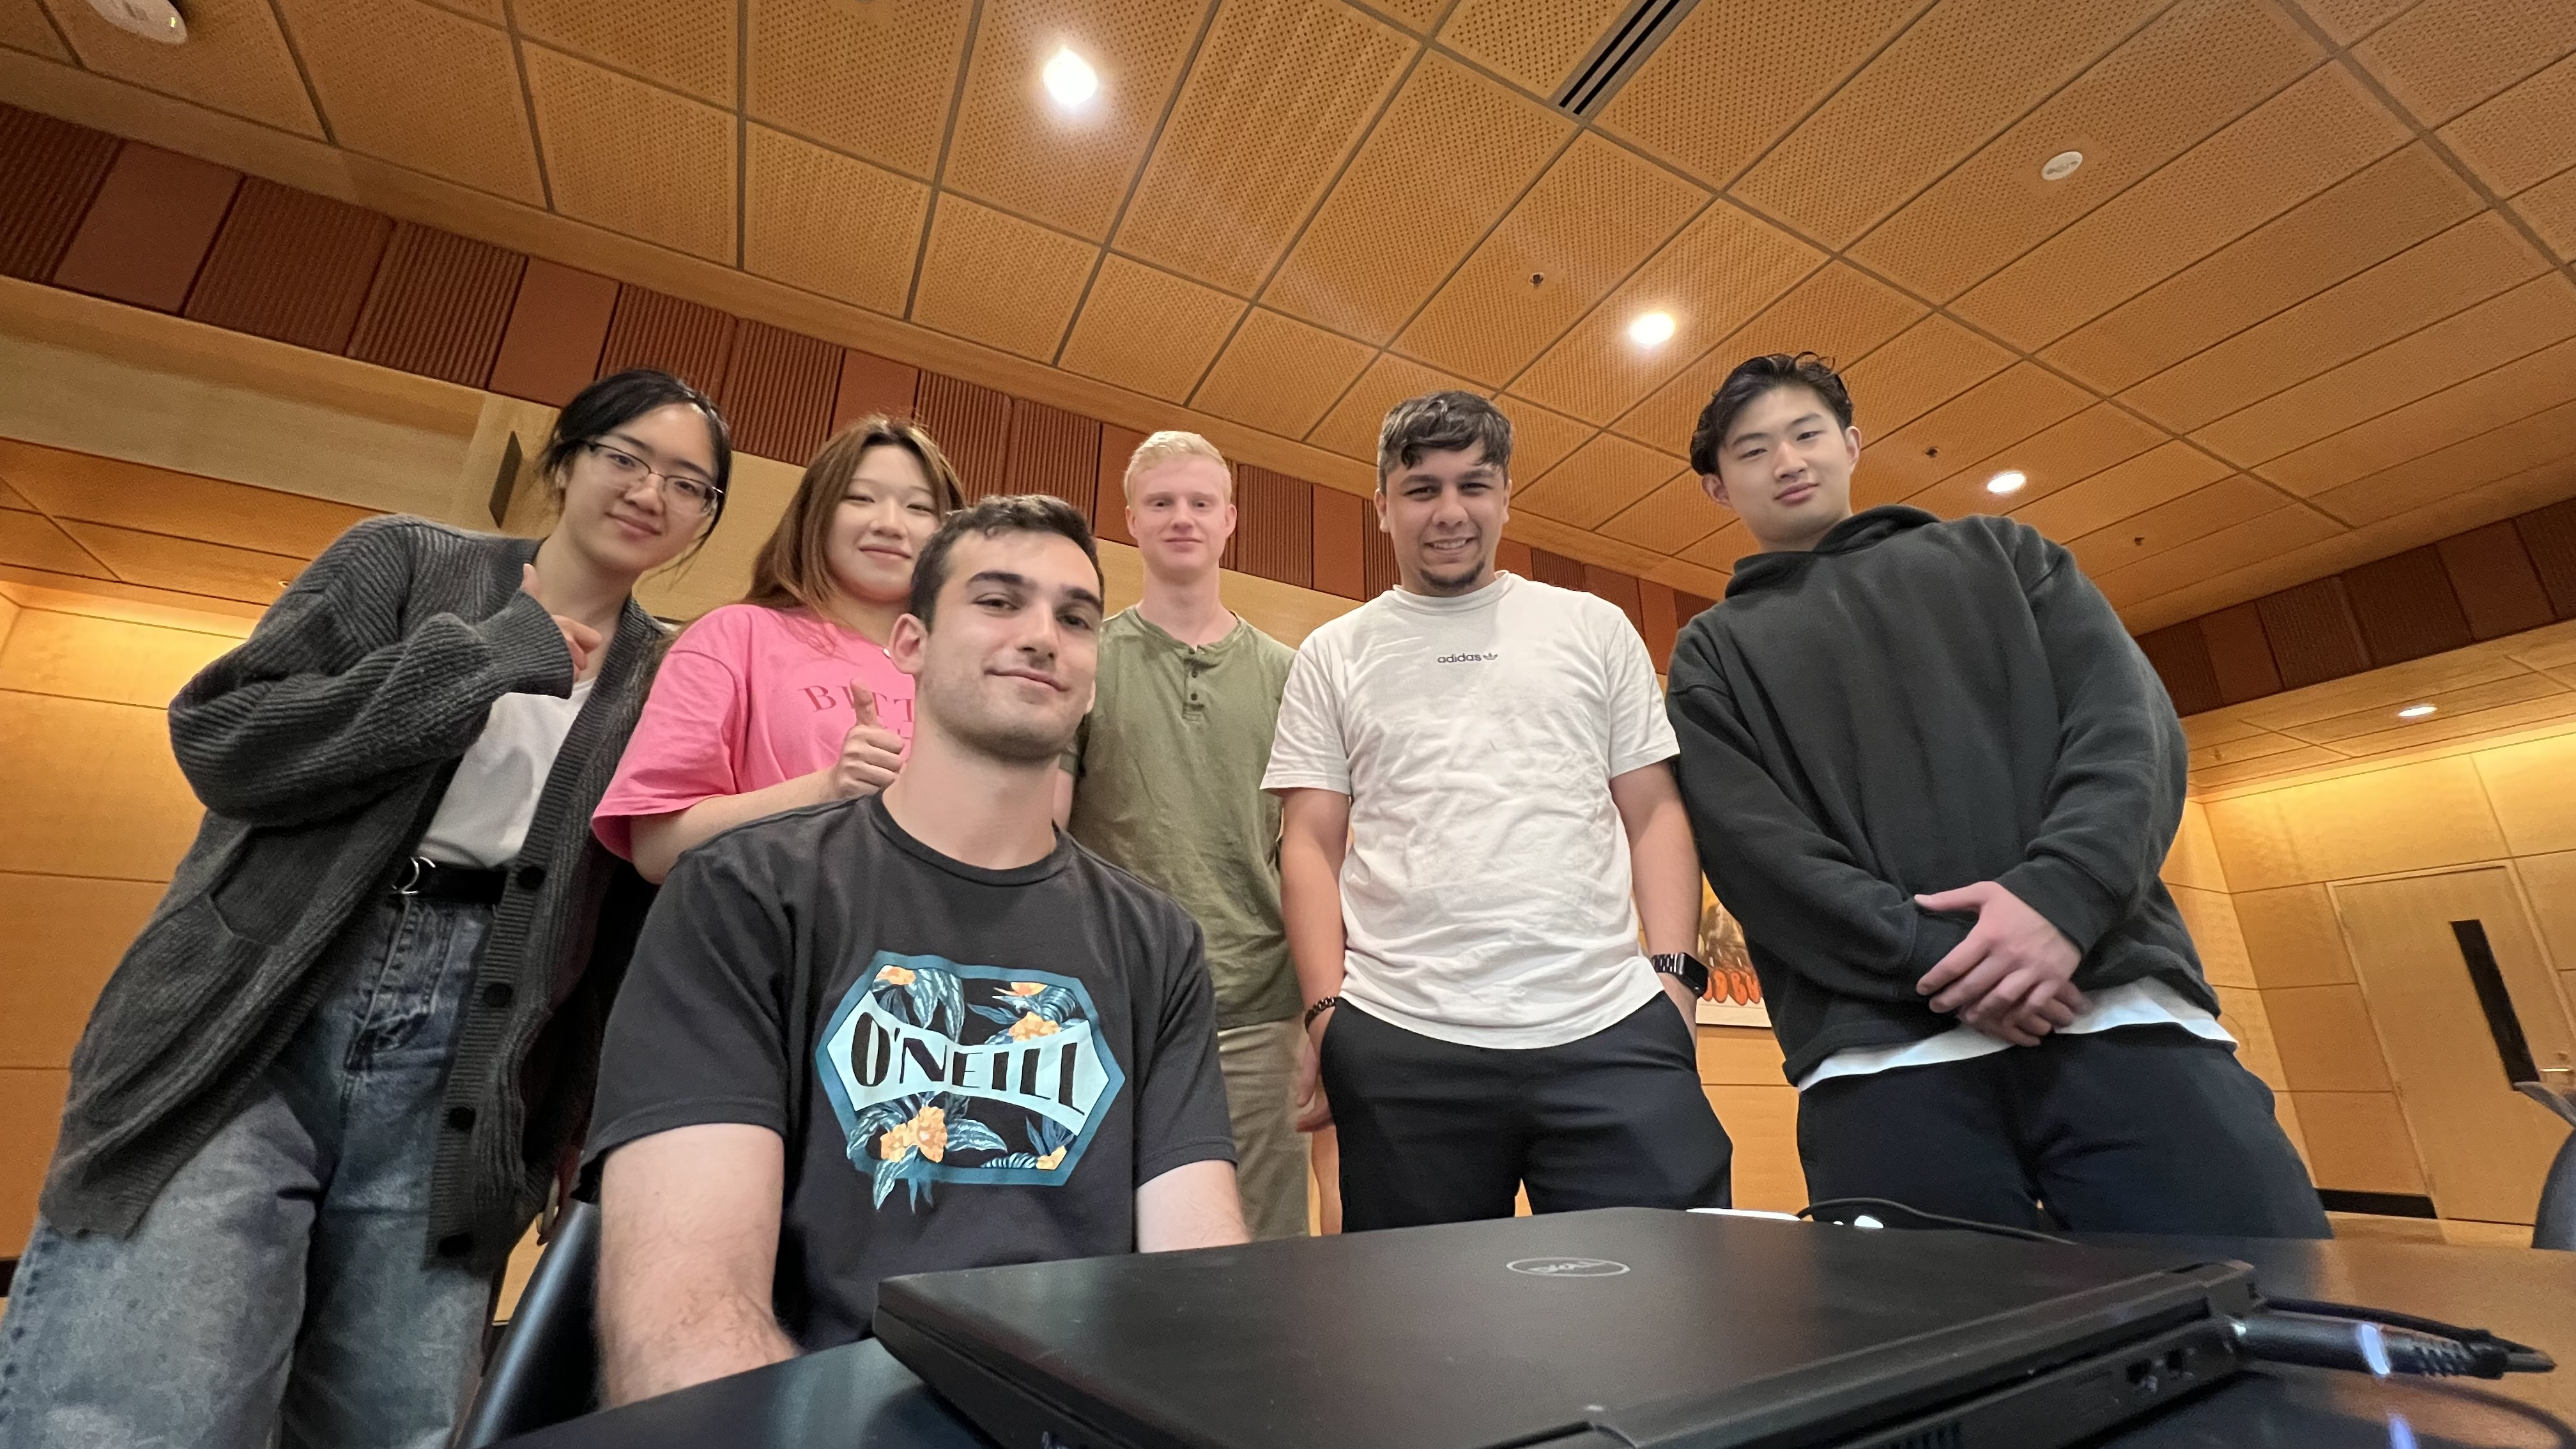
\includegraphics[width=4.04167in,height=\textheight]{Team Photo.jpg}

Our team, \textbf{Team Steve}, is driven by Steve's desire for a website that describes how new AI Tools are used in the recruitment process. For context, Steve (as seen in the black O'Neill shirt in the front left) is a student here at the Stephen M. Ross School of Business who is NOT in our project team. When deciding our team name, we thought it'd be a great idea to name it after the first person we encounter. We happened to run into Steve outside of our classroom, and the rest is history.

\hypertarget{jingyi-wang}{%
\section{Jingyi Wang}\label{jingyi-wang}}


\includegraphics[width=2.16667in,height=\textheight]{Vera Photo.png}

\textbf{Background}

My name is Jingyi (Vera) Wang, currently a Master of Business Analytics student at the University of Michigan Ross School of Business. In May 2023, I graduated from Boston University with a concentration in Finance and Business Analytics. From my previous academic and internship experiences, I found my passion for business analytics. That's the reason why I decided to pursue a graduate degree in order to help me specialize in my area of interest and enrich my experience and knowledge in the field.

\textbf{Experience}

My experience is mainly composed of internships, projects, and case competitions. In 2021, I interned at Accenture as a management consulting intern. I managed project plans, conducted data analysis, and facilitated platform testing sessions for clients to improve the efficiency and accuracy of their online platform. In 2022, I interned at Vantage House Media as a finance intern. I generated comprehensive financial reports and provided stakeholders with valuable recommendations and potential VC prospects based on data analysis. In addition, I was a quantitative financial analyst intern at Shenwan Hongyuan Securities, where I built python models to select top-performing stocks and assess fund managers' performance.~

\textbf{Fun Facts}

\begin{itemize}
\item
  I have two pet guinea pigs
\item
  I never watch horror movies
\item
  I love photography, and I have previously operated a photography social account of my own
\end{itemize}

\hypertarget{kuigang-zhang}{%
\section{Kuigang Zhang}\label{kuigang-zhang}}

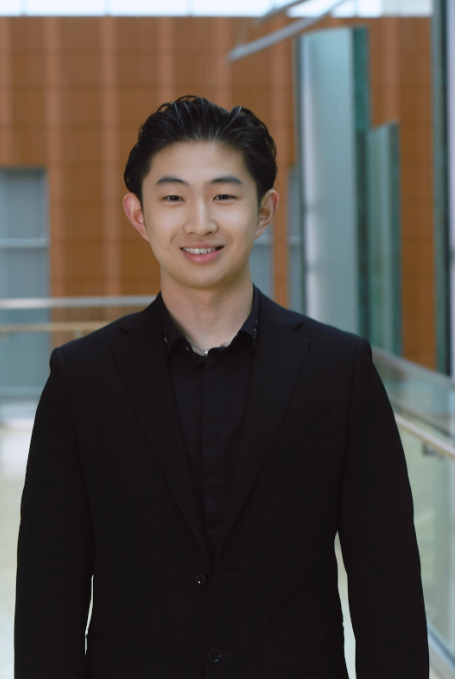
\includegraphics[width=2.1875in,height=\textheight]{KG Photo.png}

\textbf{Background}

My name is Kuigang Zhang, and I go by KG. I graduated from UCLA with a Data Science major and an Accounting minor in June 2023. Programming and business have been two areas that I am passionate about; therefore, I decided to pursue a Master of Business Analytics here at the University of Michigan Ross School of Business. I look forward to enriching my toolbox, meeting like-minded people, and getting the most out of the program.

\textbf{Experience}

I have four years of experience in programming, and have completed a number of Kaggle Competition as well as machine learning projects, and I have worked as an data analyst intern at the Shanghai Research Institute of Building Science Academy, where I enabled household energy consumption forecast in Shanghai for managing and planning urban energy utilization, covering a wide range of locations and building types.I have also worked as a data analyst intern at Lin Zhen Trading, where I developed an integrated data-driven retail supply chain management app in support of the bedding items business.

\textbf{Fun Facts}

\begin{itemize}
\item
  I was born and raised in Africa
\item
  I can deadlift 400lbs
\item
  I speak 5 languages
\end{itemize}

\hypertarget{michael-czapp}{%
\section{Michael Czapp}\label{michael-czapp}}

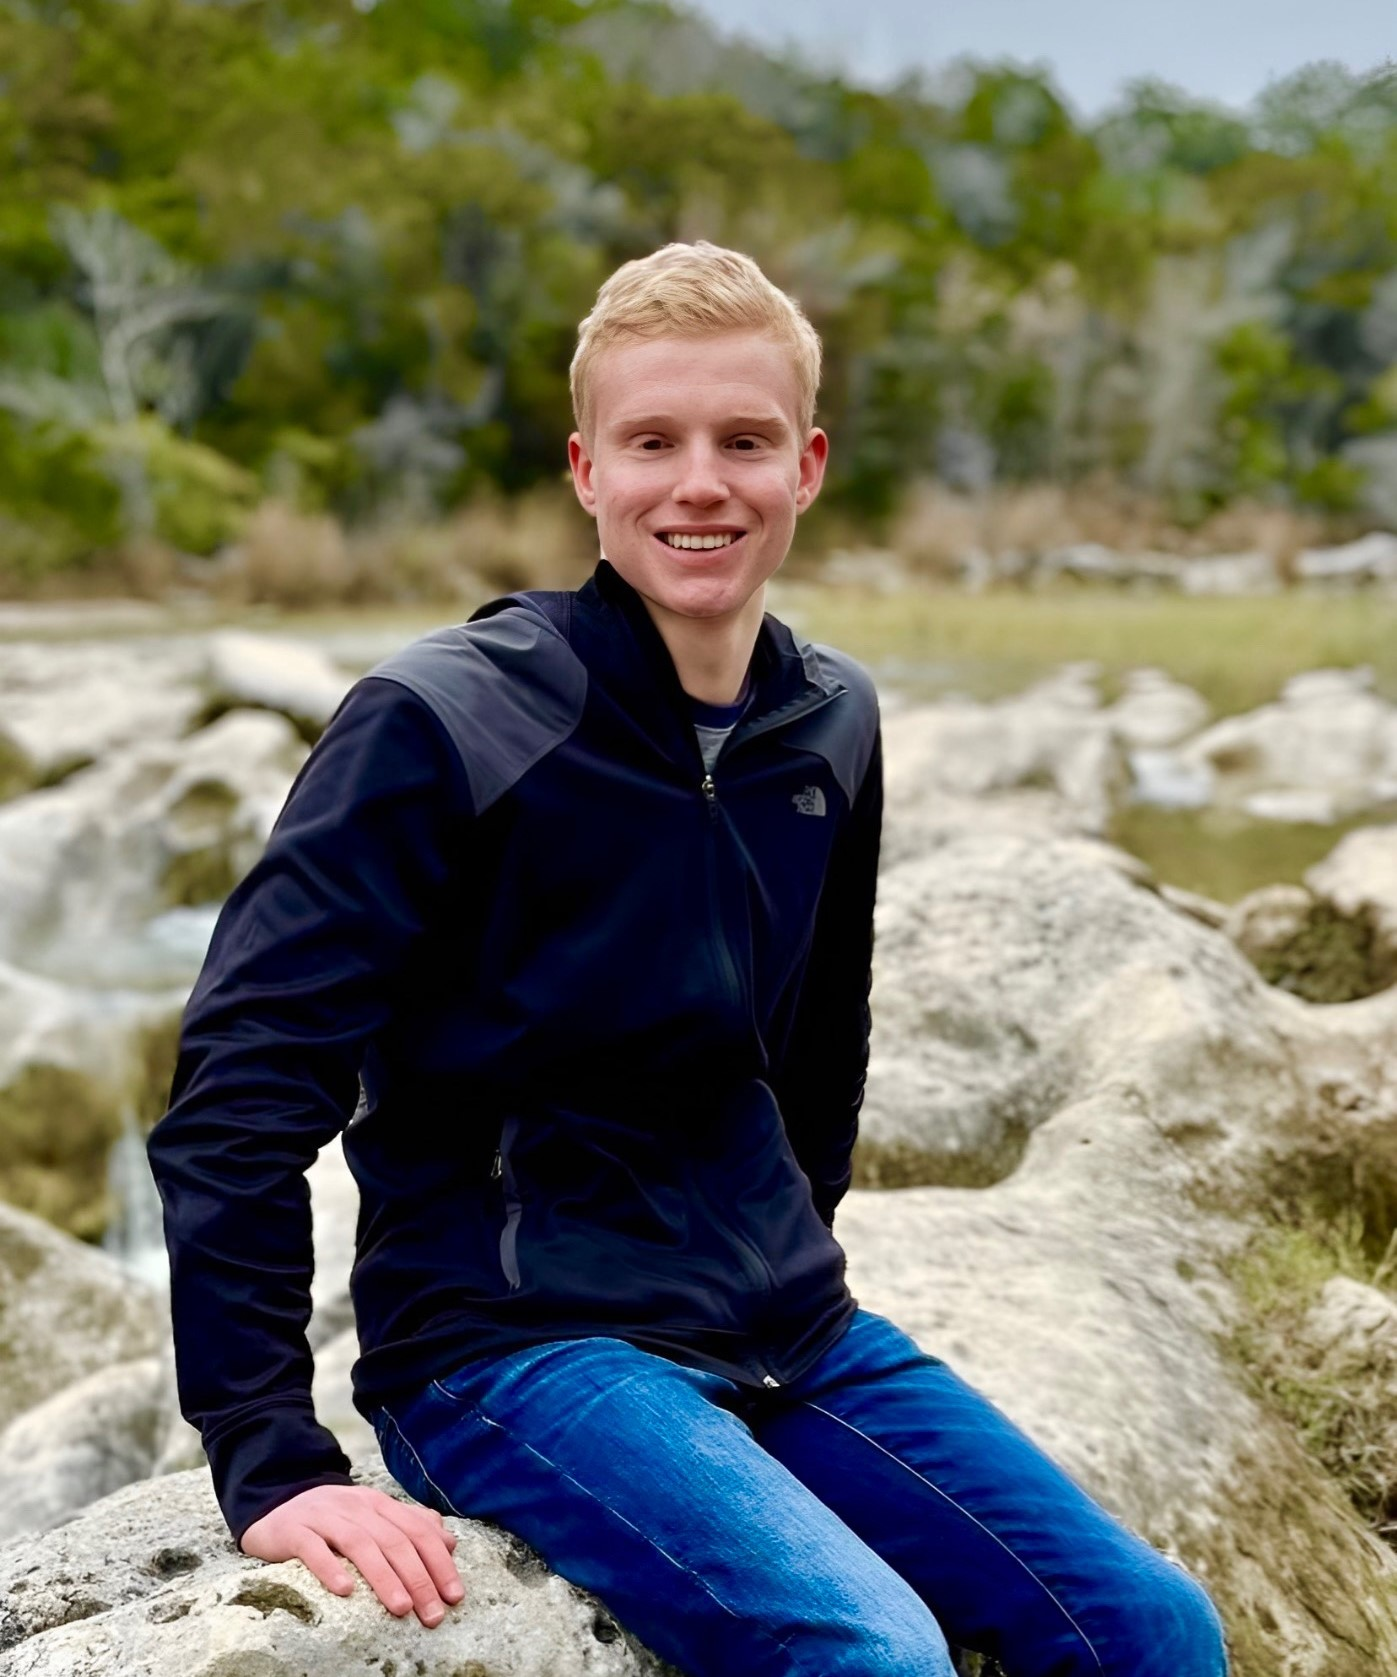
\includegraphics[width=2.36458in,height=\textheight]{Michael Czapp Photo.jpeg}

\textbf{Background}

My name is Michael Czapp, and I am currently a Master of Business Analytics (MBAn) student at the University of Michigan Ross School of Business. In April 2023, I graduated from the College of Engineering here with a Bachelor of Science in Industrial \& Operations Engineering. I knew I wanted to specialize in analytics, so starting a graduate program right after graduation made the most sense. It also allowed me to have an extra year at the University of Michigan and stay in my home state, and I plan to make the most of it!

\textbf{Experience}

My experience primarily consists of two summer internships. In 2021, I interned at DTE Energy in Detroit, MI as a Continuous Improvement Intern. I got to develop Power BI dashboards, lead a time study analysis on claim investigations, and support the execution of a pilot study at one of the company's sites. In 2022, I interned at Boston Scientific Corporation as a Global Supply Chain Consulting Intern, which was essentially an internal consulting role. I built automations, helped plan a global virtual conference, and used Excel to identify opportunities to decrease shipping costs to customers, all of which provided me with great experience in using data to discover meaningful insights to share with stakeholders.

\textbf{Fun Facts}

\begin{itemize}
\item
  Both my older brother and sister studied industrial engineering in undergrad
\item
  I play hockey as both a goalie and a skater
\item
  I've lived in the state of Michigan for my entire life
\end{itemize}

\hypertarget{xinqian-dai}{%
\section{Xinqian Dai}\label{xinqian-dai}}

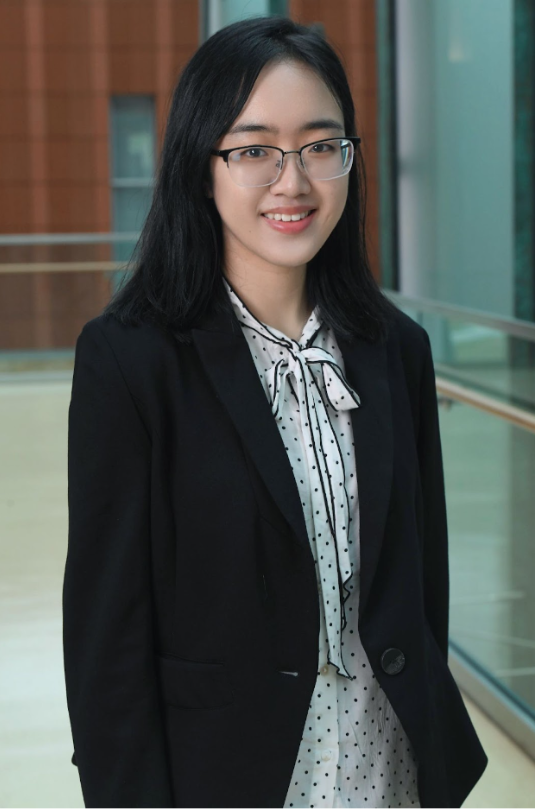
\includegraphics[width=2.08333in,height=\textheight]{Demi Photo.png}

\textbf{Background}

Hello! My name is Xinqian (Demi) Dai, and I come from the beautiful province of Heilongjiang, China, where I was born and raised. In 2019, I embarked on my exciting journey by enrolling at the University of Massachusetts Amherst for my undergraduate studies. I graduated with a double major in Marketing and Statistics in May 2023. My interest in Marketing has deep roots that extend back to my childhood days when I found myself more fascinated by the commercial inserts of a washing powder than the animated series on TV.~ Currently, I am intrigued by Customer Analytics, Advertising Effectiveness, and Digital Marketing, and I'm eager to delve deeper into these areas. Looking ahead, my post-graduation aspirations involve entering into the MarTech (Marketing Technology) industry. Armed with the knowledge and skills from the MBAn program, I aim to make a significant impact by applying data-driven strategies and innovative marketing technologies.

\textbf{Experience}

During my time at UMass Amherst, I engaged in a diverse range of research experiences and marketing projects. As a Marketing Research Assistant at the UMass Ombuds Office, I analyzed data from over 300 undergraduate student visitors, studying variables like gender and major to identify successful conflict resolution strategies. Utilizing R and Python, I applied regression models to estimate meeting times and understand the impact of visitor demographics on appointment durations. During my participation in the Research Experiences for Undergraduates (REU) Program, I conducted full-time research on Bayesian parameter estimations, highlighting the effectiveness of Bayesian models over traditional linear regression models. Additionally, as a Research Assistant in the UMass Marketing Department, I analyzed customer reactions to visual advertisements for various product categories and conducted experiments to evaluate the effect of different headbands on students. As a Strategist for the UMass AdLab, I designed customized questionnaires and implemented successful advertising strategies, resulting in a significant increase in orders for local companies. These experiences have shaped my passion for business analytics and my dedication to data-driven research and strategic planning.

\textbf{Fun Facts}

\begin{itemize}
\item
  A24 is my favorite film production company
\item
  I'm better at cooking than baking:))
\item
  My hometown holds the International Ice and Snow Festival every winter
\end{itemize}

\hypertarget{yousuf-altameemi}{%
\section{Yousuf Altameemi}\label{yousuf-altameemi}}


\includegraphics[width=2.38542in,height=\textheight]{Headshot.jpg}

\textbf{Background}

I was born and raised in Baghdad, Iraq, but now I live in the metro Detroit area. Besides my regular job, I love doing photography as a hobby. I enjoy capturing moments and emotions with my camera, and it lets me see the world in a whole new way. Additionally, I have a knack for analytics; I enjoy working with data, finding patterns, and gaining valuable insights from it. This analytical mindset helps me both in my photography and other aspects of life.

\textbf{Experience}

I graduated from Wayne State University in 2022 with a double major in Finance and Business Administration. For the past three years, I have been working as an IT Business Analyst at DTE Energy, where I have been involved in various analytical projects within the IT department. My responsibilities include analyzing data, identifying patterns, and providing valuable insights that contribute to the company's IT strategies and decision-making processes. I have also had the opportunity to collaborate with external consultants, showcasing my ability to work effectively with diverse teams and stakeholders. With a strong analytical mindset and a background in finance and business, I am well-equipped to contribute positively to any project or team I am a part of.

\textbf{Fun Facts}

\begin{itemize}
\item
  I am a part-time photographer, I shoot portraits, events and weddings
\item
  I enjoy playing soccer, my friends and I play twice a week
\item
  I collect vintage Ralph Lauren clothing
\end{itemize}

\hypertarget{what-is-artificial-intelligence-ai}{%
\chapter{What is Artificial Intelligence (AI)?}\label{what-is-artificial-intelligence-ai}}

Artificial intelligence is the simulation of human intelligence processes by machines, especially computer systems. Specific applications of AI include expert systems, natural language processing, speech recognition and machine vision (1).

The functioning of AI involves the processing of extensive labeled training data, identifying correlations and patterns within the data, and using these patterns to make predictions about future states. For instance, a chatbot can learn to produce lifelike conversations with people after being trained on text examples, while an image recognition tool can accurately identify and describe objects in images through the analysis of millions of examples. Generative AI techniques have also shown significant progress in generating realistic text, images, music, and other media.

AI programming revolves around cognitive skills that encompass:

\textbf{1. Learning:} The acquisition of data and creation of algorithms that convert it into actionable information, providing step-by-step instructions for specific tasks to computing devices.

\textbf{2. Reasoning:} The selection of appropriate algorithms to achieve desired outcomes.

\textbf{3. Self-correction:} Continuously refining algorithms to ensure optimal and precise results.

\textbf{4. Creativity:} Utilizing neural networks, rules-based systems, statistical methods, and other AI techniques to generate novel images, text, music, and ideas.

The significance of artificial intelligence lies in its potential to revolutionize how we live, work, and engage in leisure activities. AI has found effective applications in automating tasks traditionally performed by humans, such as customer service, lead generation, fraud detection, and quality control. Particularly in repetitive and detail-oriented tasks, AI often outperforms humans in terms of speed and accuracy, as demonstrated in analyzing vast numbers of legal documents for accurate field completion. The processing capabilities of AI enable enterprises to gain valuable insights into their operations that were previously inaccessible.

The proliferation of AI tools, especially generative AI, promises transformative impacts across various domains, including education, marketing, and product design. Leading companies like Alphabet, Apple, Microsoft, and Meta have integrated AI technologies to enhance their operations and maintain a competitive edge. For instance, Google, a subsidiary of Alphabet, employs AI at the core of its search engine, Waymo's self-driving cars, and Google Brain, the pioneer behind the transformer neural network architecture that drives recent advancements in natural language processing.

Overall, the advent of AI not only drives efficiency improvements but also creates unprecedented business opportunities, as evidenced by Uber's success in leveraging computer software to connect riders with taxis and becoming a Fortune 500 company. The ongoing progress in AI holds the potential to shape a dynamic and transformative future across various industries.

\hypertarget{ai-tools-for-job-searching}{%
\chapter{AI Tools for Job Searching}\label{ai-tools-for-job-searching}}

A very crucial part of the recruiting process is finding the right job. With numerous platforms for companies to post jobs and the company's career pages themselves, it may seem like there are too many to choose from. In addition to this, it may be difficult to find exactly what you're looking for. The following three sections discuss some popular tools you can use to narrow your search and identify the best job for you!

\hypertarget{talentprise}{%
\section{Talentprise}\label{talentprise}}

\href{https://www.talentprise.com/}{Talentprise} is revolutionizing the way job seekers approach their career aspirations. In a world where standing out amidst a sea of applicants is increasingly challenging, Talentprise offers a dynamic platform that simplifies and invigorates the job search process. With a global reach, Talentprise empowers job seekers to expand their horizons, connecting them with coveted positions from local, regional, and international Fortune 500 companies. No longer confined by geographical limitations, candidates can showcase their unique value propositions and directly capture recruiters' attention. Uncover hidden job opportunities that align with your ambitions and secure the role you deserve.

In a landscape inundated with resumes and cover letters, Talentprise stands as a beacon of efficiency and innovation. By harnessing both qualitative data and the prowess of artificial intelligence, the platform empowers candidates to seamlessly rise above the competition.

Talentprise's comprehensive approach provides numerous advantages:

1. \textbf{Personalized Insights}: Take an enlightening skills assessment that reveals your strengths and areas for growth in your job-seeking journey.

2. \textbf{Total Privacy}: Retain control over your personal information, deciding who gains access to your profile and safeguarding the confidentiality of your job search.

3. \textbf{Industry Intelligence}: Stay ahead of the curve by accessing key industry trends, enabling you to adapt and elevate your chances of securing your desired role.

4. \textbf{Timely Notifications}: Never miss out on potential dream job opportunities

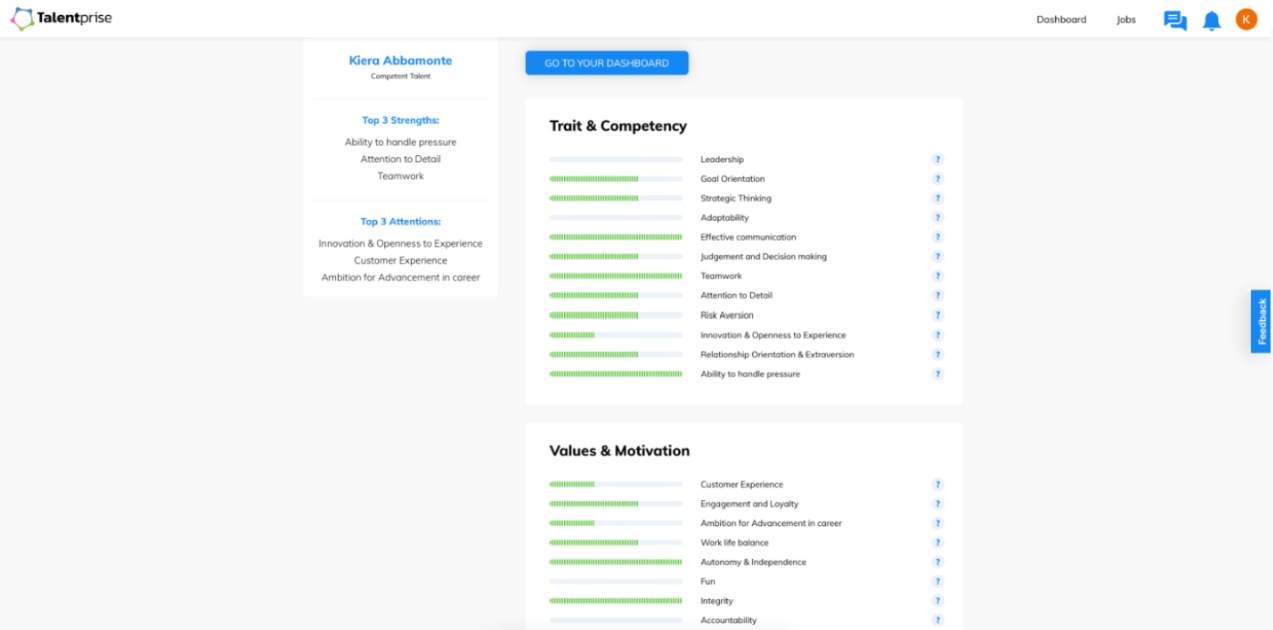
\includegraphics[width=4.63542in,height=\textheight]{talentprise1.png}

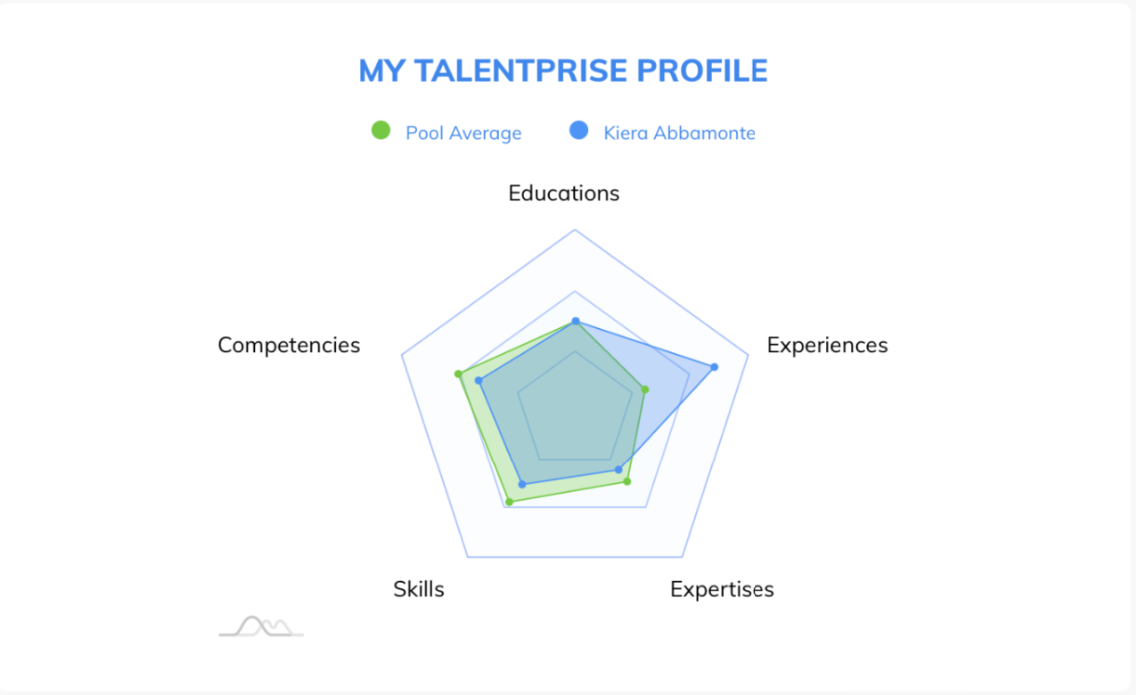
\includegraphics[width=4.54167in,height=\textheight]{talentprise 2.png}

\hypertarget{pyjama-jobs}{%
\section{Pyjama Jobs}\label{pyjama-jobs}}

\href{https://www.kickresume.com/pyjama-jobs/}{Pyjama Jobs} is an innovative AI-driven platform that aims to streamline the job search process by connecting job seekers with suitable employment opportunities. By harnessing the capabilities of AI, Pyjama Jobs eliminates the need for exhaustive job searching and instead allows job seekers to be effortlessly discovered by recruiters based on their skills, qualifications, and preferences.

\textbf{1. Resume Creation and Upload:} Pyjama Jobs simplifies the initial step of job searching by offering users the choice to either create a resume using the platform's resume builder or upload an existing one from other sources. This feature ensures that job seekers present a comprehensive and accurate representation of their skills and experiences.

\textbf{2. AI-Driven Matching:} The heart of Pyjama Jobs' functionality lies in its AI-driven matching algorithm. Once a user's resume is uploaded, the platform's AI analyzes the document and cross-references it against an extensive database of job openings. This process enables both the job seeker and potential recruiters to swiftly determine if there is a suitable match.

\textbf{3. Tailored Job Offers:} Job seekers using Pyjama Jobs can expect a more personalized job search experience. Recruiters only make contact with candidates who are a strong fit for a specific position, saving both parties time and effort. This personalized approach enhances the overall quality of job offers received by candidates.

\textbf{5. Global Opportunities:} Pyjama Jobs goes beyond geographical limitations by enabling job seekers to apply for remote positions worldwide. This global reach increases the breadth of opportunities available to users and reflects the evolving nature of modern work arrangements.

\textbf{6. Comprehensive Job Information:} Each job post on Pyjama Jobs includes essential details such as salary ranges, providing job seekers with crucial insights to help them make informed decisions about potential opportunities.

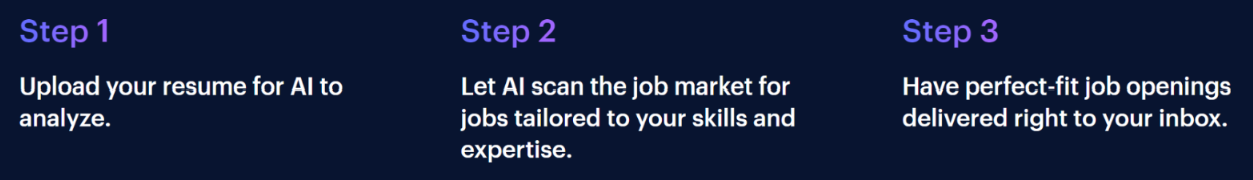
\includegraphics[width=5.66667in,height=\textheight]{pyjama jobs.png}

\hypertarget{resume-and-cover-letter-optimizers}{%
\chapter{Resume and Cover Letter Optimizers}\label{resume-and-cover-letter-optimizers}}

In today's competitive and ever-changing job market, it is crucial to have a well-crafted resume and cover letter to stand out from competitors and gain the opportunity to catch employers' attention. With the recent advancements in AI tools, students can now leverage technology to optimize their resumes and cover letters effectively. Here are some popular AI resume and cover letter builders (1) (2):

\hypertarget{resume.com}{%
\section{Resume.com}\label{resume.com}}

\href{https://www.resume.com/resume/builder/783ccdad-f0ea-4ff0-aa57-c59d6100995a}{Resume.com} is a free online resume builder that helps you create a resume tailored to your skills and experience. One outstanding feature of Resume.com is to pinpoint the most relevant keywords for your target positions to mention in the resume, which is essentially beneficial when applying for positions that require specific technical or professional skills and abilities. In addition, it also provides various customizable templates, editing tools, resume tips, and resume sample, where you could easily edit your content based on your individual needs. It also provides a resume evaluation service by giving personalized feedback on your resume.

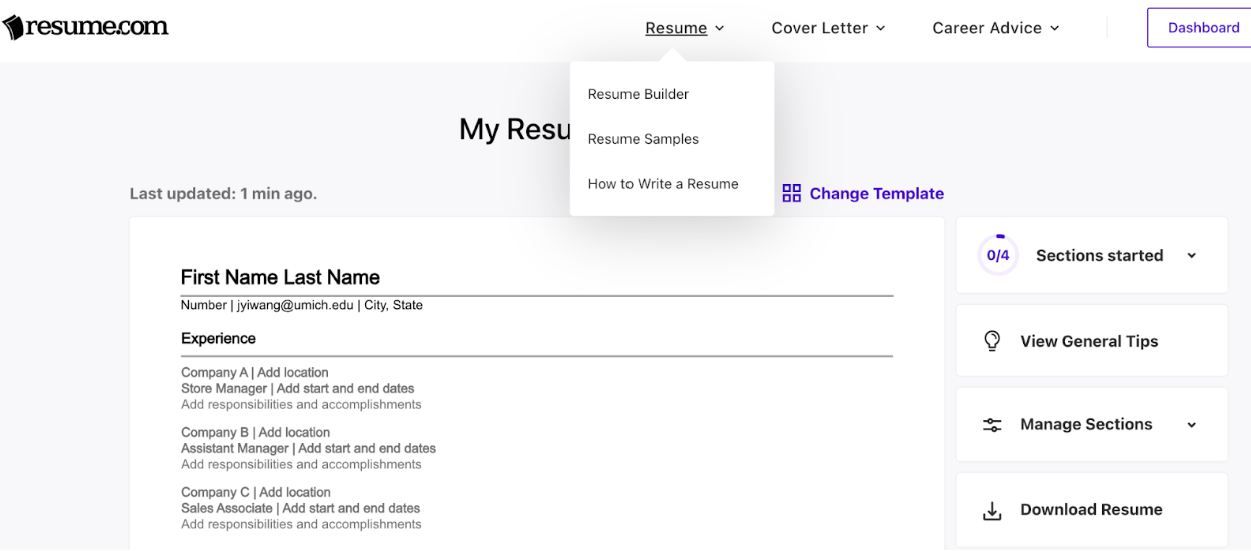
\includegraphics[width=5.90625in,height=\textheight]{Resume.com pic.png}

\hypertarget{jobscan}{%
\section{Jobscan}\label{jobscan}}

\href{https://www.jobscan.co/resume-score}{Jobscan} is a popular AI resume builder that analyzes your resume and provides suggestions for improvements based on the description and keyword (1). It has the unique feature of scanning a resume against a specific job description, offering you a detailed report about how your skills and experience are being matched with areas where you can enhance your alignment with the role. It provides a very detailed feedback report showcasing which section you should focus on by listing out your missing skills and keywords for several sections: ATS findings, recruiter findings, hard skills, and soft skills.

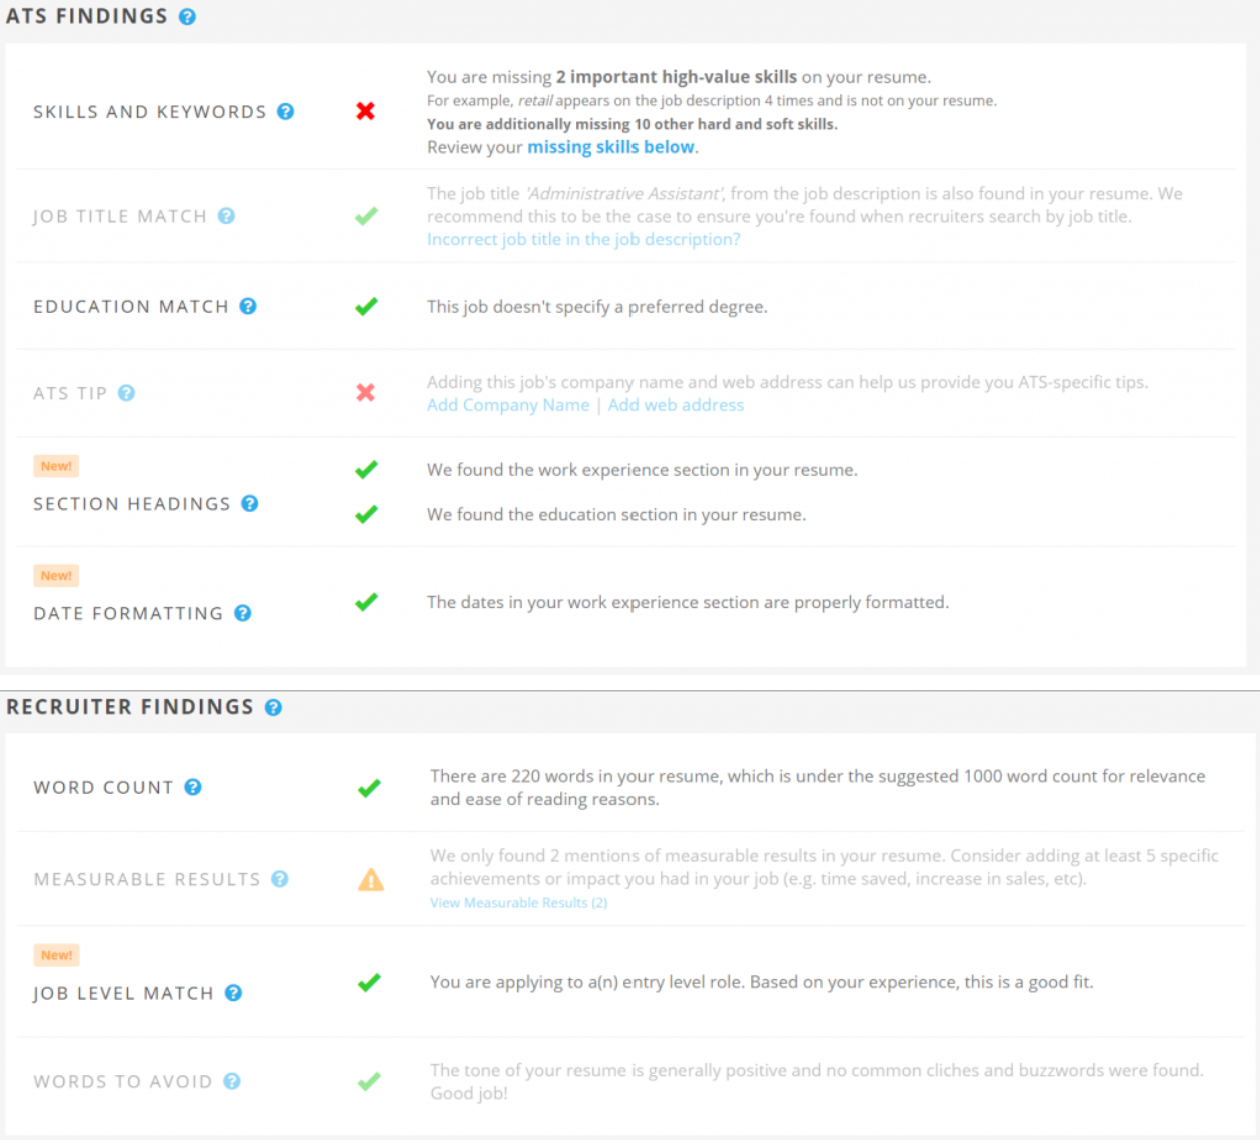
\includegraphics[width=5.11458in,height=\textheight]{Jobscan findings.png}

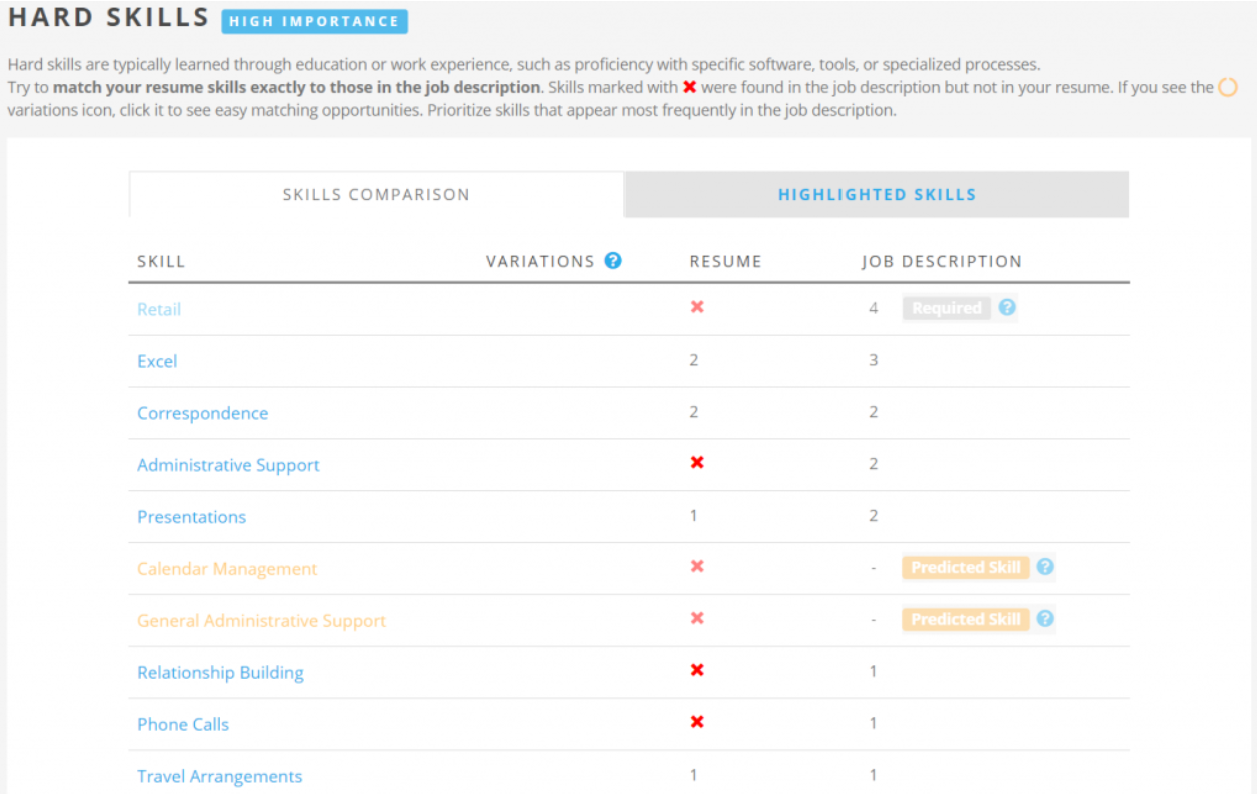
\includegraphics[width=3.98958in,height=\textheight]{Jobscan findings 2.png}

\hypertarget{kickresume}{%
\section{Kickresume}\label{kickresume}}

The modern AI resume builder \href{https://www.kickresume.com/en/}{Kickresume} makes the process from creating to checking a resume much easier than before. It includes a wide range of designer-created templates, a detail-oriented log of changes made to your resume, a drag-and-drop editor, and a easy-to-use one-click design feature (1). It generates and optimizes well-formatted professional resumes that strongly match with your personalized positions by utilizing various in-build AI tools such as spell checkers, AI text analysis, natural language processing, and style guides. In addition, Kickresume offers an unique feature that allows users to upload a video introduction as an alternative job submission method instead of traditional resume format. This video can help employers better understand your strengths and skills. All these features make Kickresume a great platform for job seekers to improve their professional credentials and create a high-quality resume in a short amount of time.

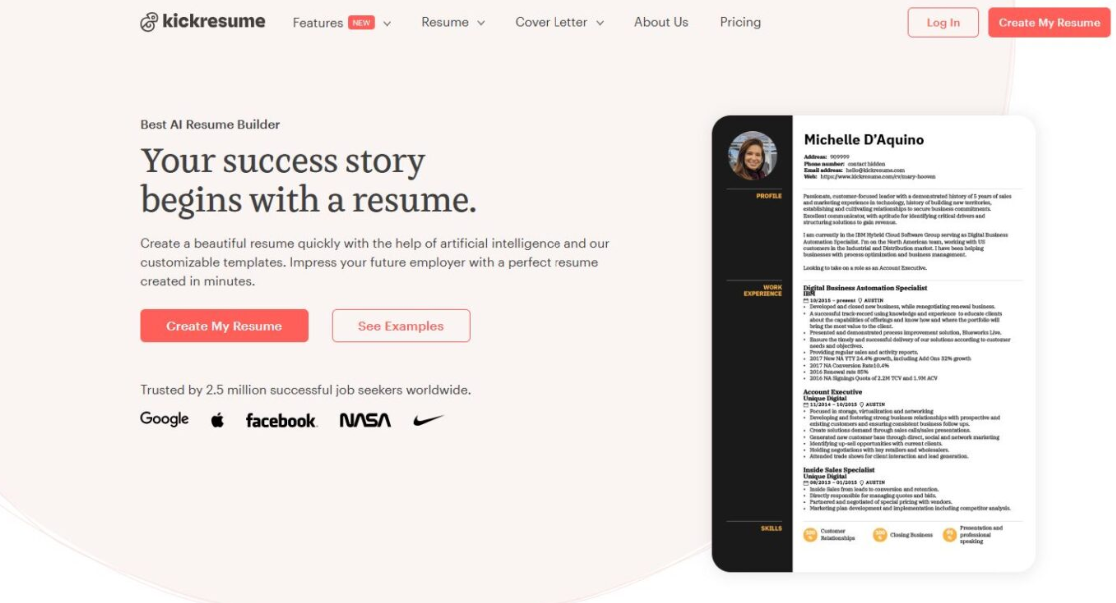
\includegraphics[width=5.46875in,height=\textheight]{Kickresume pic.png}

\hypertarget{lazyapply}{%
\section{LazyApply}\label{lazyapply}}

\href{https://lazyapply.com/cover-letter-generator}{LazyApply} is a free AI cover letter generator to help you create professional cover letters easily. It includes over 20 options of writing tones, such as humble, convincing, appreciative, formal, and inspirational, to assist you with generating the most suitable writing style for your personal cover letter (2). By simply inputting your personal details like your name, skills, the job information, and the recruiter's name to whom you want to send the cover letter, it helps you generate an appropriate cover letter fast and accurately. It also offers abundant cover letter templates based on specific organizations or job roles.

\hypertarget{rezi}{%
\section{Rezi}\label{rezi}}

\href{https://www.rezi.ai/}{Rezi} is a professional AI cover letter generator. It provides over 250+ cover letter samples, which allows job seekers to begin the process of creating cover letters (2). After analyzing your resume, Rezi makes references from your resume experiences and how they fit best for the job role in your cover letter. If you enter the ideal company details and specific skills and position highlights, Rezy will generate a tailored cover letter in seconds.~

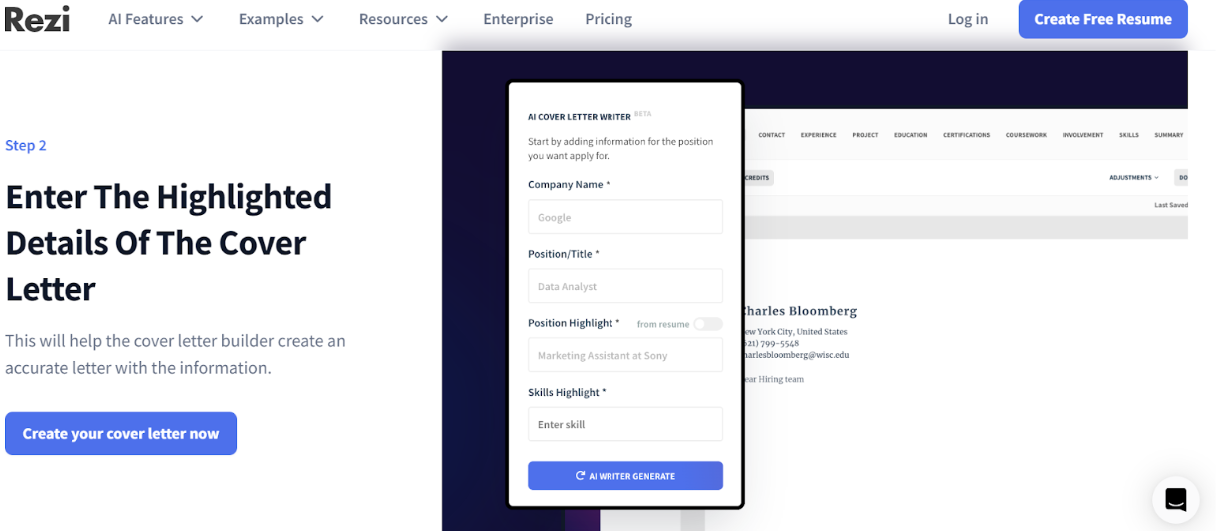
\includegraphics[width=5.5in,height=\textheight]{Rezi pic.png}

\hypertarget{cover-letter-simple.ai}{%
\section{Cover Letter Simple.ai}\label{cover-letter-simple.ai}}

\href{https://coverlettersimple.ai/}{Cover Letter Simple.ai} is unique from other cover letter tools mentioned above as it focuses on generating unique and job-specific cover letters. After entering your ideal job title, it searches billions of data points to retrieve relevant information for the job, such as expected skills and accomplishments (2).

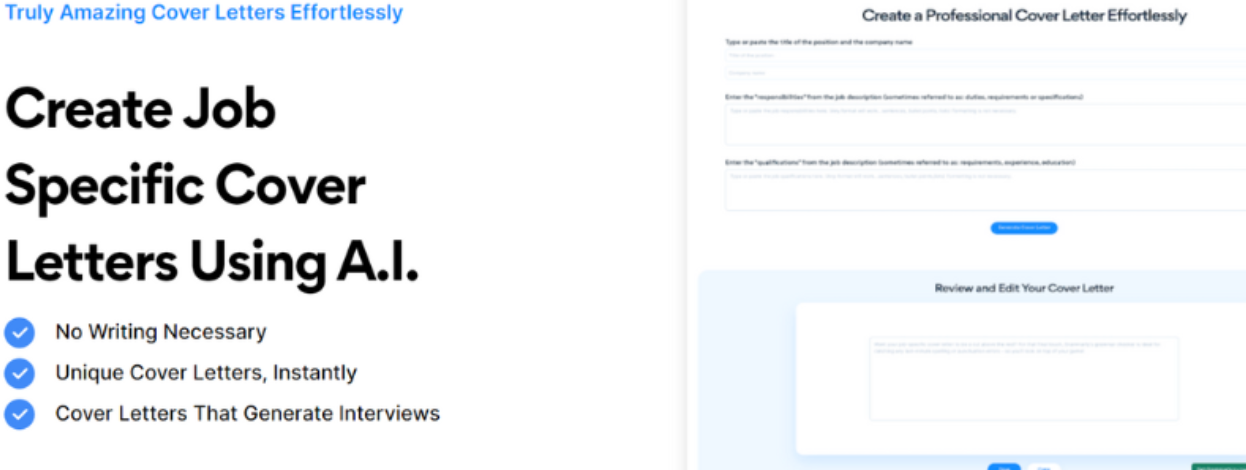
\includegraphics[width=6.80208in,height=\textheight]{coverlettsimpleai pic.png}

\hypertarget{student-practice-interviews}{%
\chapter{Student Practice Interviews}\label{student-practice-interviews}}

Effective interview preparation is essential for students to improve their interview skills and achieve their career goals in the long term. With the evolution of AI, many interview practice AI tools are introduced to simulate real interview scenarios to help students hone communication skills. In this section, we will delve into a few AI-powered interview practice tools that help students stand out from other candidates.

\hypertarget{standout}{%
\section{Standout}\label{standout}}

\href{https://standout.com/}{Standout} is a mock interview practice platform for job seekers to prepare for and practice for interviews. Its unique Intelligent Mirror™ technology provides users with personalized AI feedback of verbal behaviors, non-verbal behaviors, and communication missteps to help you reflect on your performance. Users can record, review, and re-record interview answers to various interview questions. Following the video recording, StandOut will analyze responses for hesitations, enunciations, and response timing to provide feedback on interviewing skills.

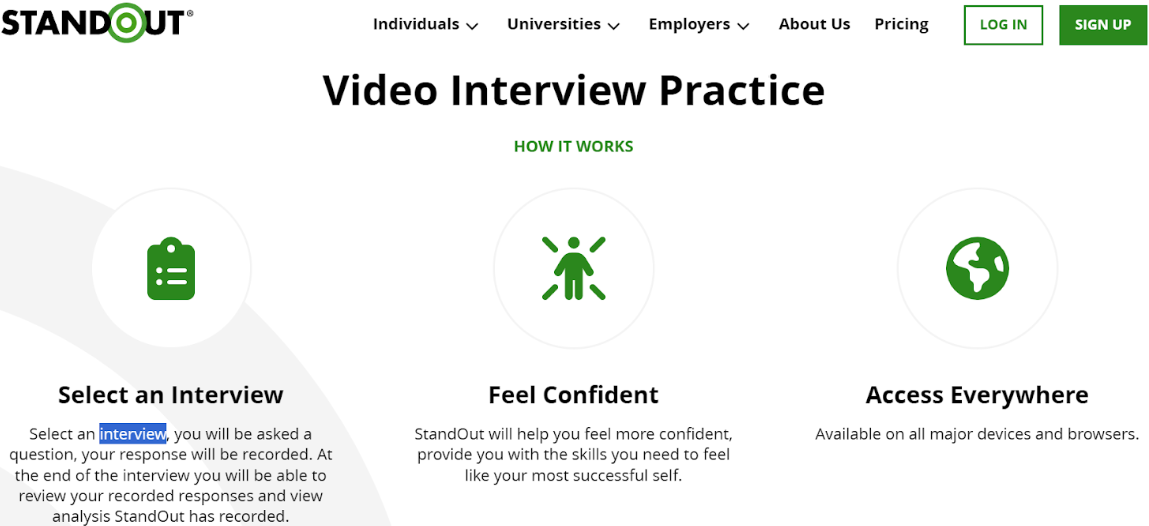
\includegraphics[width=4.64583in,height=\textheight]{standout pic.png}

\hypertarget{yoodli}{%
\section{Yoodli}\label{yoodli}}

\href{https://app.yoodli.ai/}{Yoodli} is an AI-powered communication coach for job seekers to practice interviews and enhance interview skills. Besided general interview answer evaluations, Yoodli can evaluate users' speaking patterns, speech, and body language. Users can find out exactly how fast or slow you speak, if your word choice can be improved, and which filler words you use (and how often), among other insights (1). After uploading videos, users will get coaching comments and actionable feedback with a summary of the video's main points. Additionally, it offers a library of mock interview question with various categories, such as general, marketing, and consulting. You could even practice interview questions at random by using the ``Surprise Me'' function.

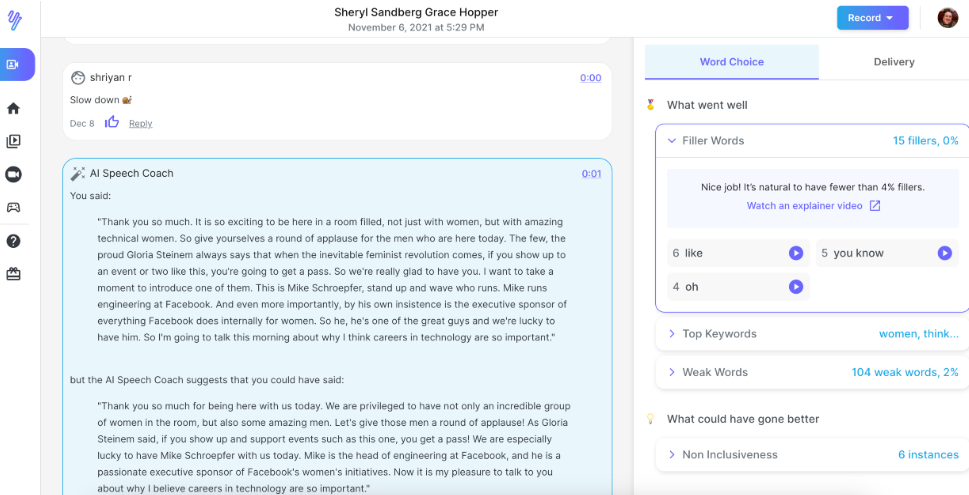
\includegraphics[width=4.85417in,height=\textheight]{yoodli pic 1.png}

Yoodli also has an innovative feature called \textbf{Private Yoodli}, which allows Yoodli to discreetly join your virtual meetings as a personal speech coach (1). It will provide feedback on your expression, clarity, and delivery during meetings to improve your overall communication skills.


\includegraphics[width=4.28125in,height=\textheight]{yoodli pic 2.png}

\hypertarget{interviewgpt.ai}{%
\section{InterviewGPT.ai}\label{interviewgpt.ai}}

\href{https://interviewgpt.ai/}{InterviewGPT.ai} is an AI-powered job interview preparation tool. By using InterviewGPT.ai, users can practice interviews for specific job roles and improve their technical skill sets (2). In addition, the tool also provides access to RecruitGenius.ai and CareerGPT.ai. The former is used by recruiters to find suitable candidates for open positions, while the latter is for candidates to explore career opportunities and paths (2).

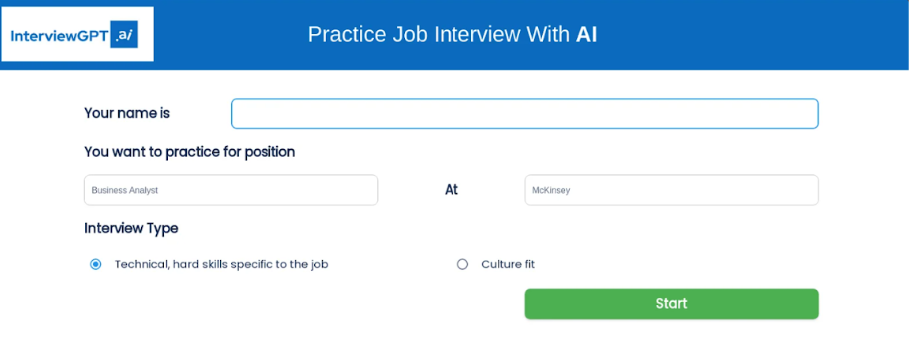
\includegraphics[width=4.90625in,height=\textheight]{intergptai pic.png}

\hypertarget{automated-applications}{%
\chapter{Automated Applications}\label{automated-applications}}

With an overwhelming amount of job postings across countless platforms and websites, it can be stressful and time consuming to apply to each individually. Thus, you can leverage AI tools that can automate your application process and save you precious time!

\hypertarget{teal}{%
\section{Teal}\label{teal}}

\href{https://www.tealhq.com/tools/autofill-job-applications}{Teal} offers a comprehensive autofill functionality designed to revolutionize job search process. By simply installing Teal's free Chrome extension from the Google Chrome Web Store, users gain access to a range of powerful features. Seamlessly uploading their resume or LinkedIn profile into the AI Resume Builder sets the stage for a seamless experience. With the ability to automatically detect job applications across nearly 50 diverse job boards, Teal empowers job seekers to save valuable time and apply for roles swiftly. The true magic of Teal's autofill feature unfolds after saving a desired job opportunity. With just a click, users can harness the power of Teal's AI to effortlessly respond to various application questions, whether they're as straightforward as providing a ``first name'' or as complex as explaining ``Why do you want to work here?''

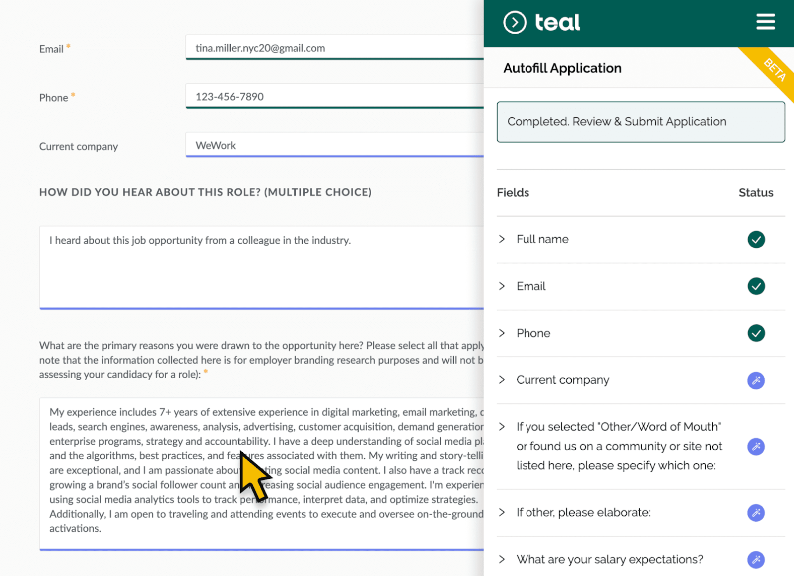
\includegraphics[width=4.125in,height=\textheight]{teal pic.png}

\hypertarget{simplify}{%
\section{Simplify}\label{simplify}}

\href{https://simplify.jobs/autofill\#how-it-works}{Simplify} was born out of the founders' personal experiences and had been applied to countless positions during their college years. Simplify serves as a dedicated job assistant, guiding users through each stage---from tailored job exploration to effortless one-click applications with the Simplify Copilot extension to seamless application tracking via a personalized dashboard. Presently, many users entrust Simplify with their recruitment endeavors, leading to an impressive five million job applications managed within a year.~

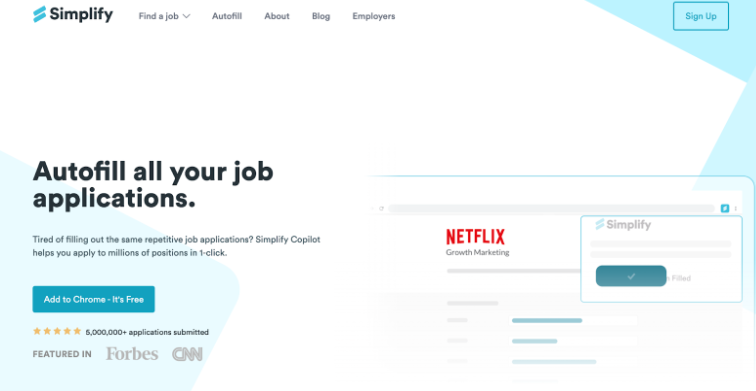
\includegraphics[width=3.88542in,height=\textheight]{simplify pic.png}

\hypertarget{lazyapply-1}{%
\section{LazyApply}\label{lazyapply-1}}

\href{https://lazyapply.com/}{LazyApply} amalgamates multiple job boards, including Linkedin, Indeed, and Ziprecruiter, within a singular dashboard, and offers a unified platform for a comprehensive job hunting experience.

Particularly noteworthy is LazyApply's Linkedin Job application bot, replete with an array of remarkable features and filters. Job seekers gain the ability to meticulously customize their search, handpicking desired skills, preferred job locations, and the number of applications to submit in a single session. The bot's proficiency extends to refined job filtering, encompassing parameters such as location, salary, posting date, experience level, industry, job title, and remote or onsite work options.~

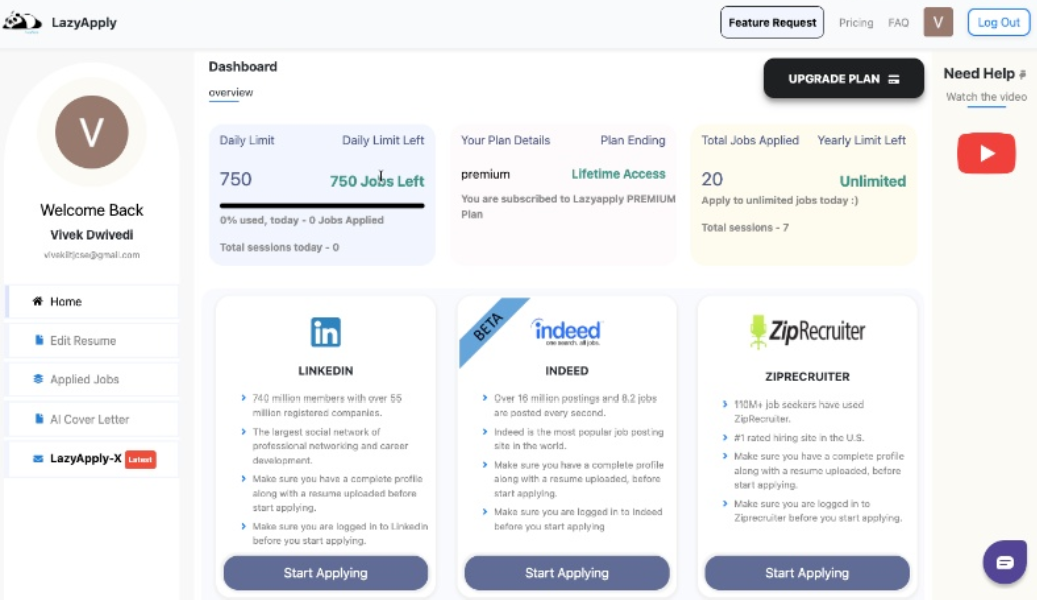
\includegraphics[width=3.85417in,height=\textheight]{lazyapply pic 2.png}

\hypertarget{what-are-applicant-tracking-systems-ats}{%
\chapter{What Are Applicant Tracking Systems (ATS)?}\label{what-are-applicant-tracking-systems-ats}}

\begin{quote}
\emph{\textbf{``}\href{https://medium.com/swlh/90-of-fortune-500-companies-use-an-applicant-tracking-system-whats-it-5a6b6d25e5e7}{More than 90\% of Fortune 500 companies} are currently using an applicant tracking system to better attract and convert top talent today.'' (1)}
\end{quote}

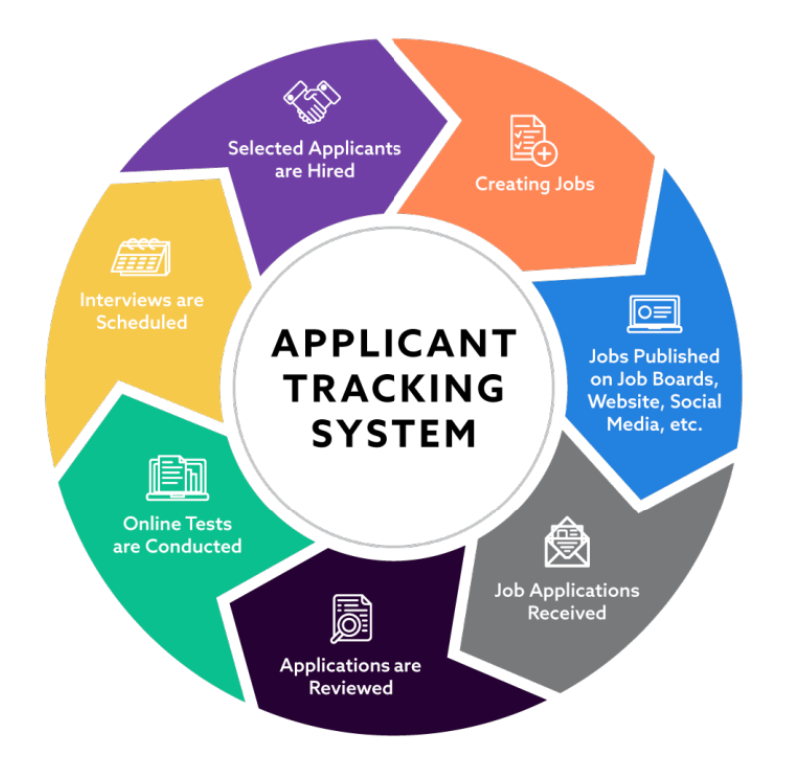
\includegraphics[width=4.08333in,height=\textheight]{ats pic.png}

\hypertarget{definition}{%
\section{Definition}\label{definition}}

An \textbf{Applicant Tracking System (ATS)} is an innovative software solution that digitally manages and automates the recruitment process. It provides a structured framework for employers to post job openings, gather candidate applications, screen resumes, schedule interviews, and ultimately select the best-fit candidates for various positions. ATS platforms serve as a comprehensive repository for all candidate-related data and communication, facilitating efficient collaboration among recruitment teams.

\hypertarget{features}{%
\section{Features}\label{features}}

An ATS is equipped with a range of features that enhance recruitment efficiency and effectiveness. Some of these features include:

\begin{itemize}
\item
  \textbf{Job Posting:} ATS software enables seamless job posting across a variety of job boards, expanding the reach of recruitment efforts and attracting a diverse pool of candidates.
\item
  \textbf{Branded Careers Page:} An ATS simplifies the creation and maintenance of a branded careers page on a company's website, enhancing its appeal to potential candidates.
\item
  \textbf{Candidate Tracking and Management:} ATS platforms automatically filter and organize candidate applications based on predefined criteria, ensuring that recruiters focus on the most relevant profiles.
\item
  \textbf{Interview Scheduling:} ATS systems facilitate efficient interview scheduling by allowing candidates to choose interview slots online, reducing the need for manual coordination.
\item
  \textbf{Workflow Management:} The ATS streamlines the entire recruitment workflow, from application submission to final selection, ensuring a consistent and structured process.
\end{itemize}

\hypertarget{benefits}{%
\section{Benefits}\label{benefits}}

An ATS offers numerous benefits that contribute to a more effective and streamlined recruitment process. These benefits include:

\begin{itemize}
\item
  \textbf{Precise Candidate Matching:} ATS platforms help identify candidates who closely match the job requirements, leading to improved candidate selection and higher retention rates.
\item
  \textbf{Accelerated Hiring Process:} By automating resume screening and candidate management, ATS systems significantly reduce the time taken to identify and hire suitable candidates.
\item
  \textbf{Cost Efficiency:} Compared to traditional recruitment methods, ATS solutions offer a cost-effective approach to talent acquisition, saving companies money on advertising and other recruitment expenses.
\item
  \textbf{Enhanced Application Relevance:} The ATS filters out irrelevant applications, ensuring that recruiters focus on high-potential candidates who align with the job criteria.
\item
  \textbf{Building High-Performing Teams:} Leveraging an ATS empowers organizations to build successful teams, as evidenced by the adoption of this technology by 90\% of Fortune 500 companies.
\end{itemize}

\hypertarget{recruiting-chatbots}{%
\chapter{Recruiting Chatbots}\label{recruiting-chatbots}}

Recruiting chatbot is an automated system that works through pre-programmed responses or artificial intelligence without a human operator. Recruiting chatbots, also known as HR chatbots, are revolutionizing the recruitment process by automating tasks like screening candidates, answering FAQs, scheduling interviews, and guiding onboarding. Designed to enhance efficiency and consistency, these bots are available 24/7 and can be a cost-effective solution for organizations.

Moreover, chatbots are continually improving in sophistication. Surprisingly, \textbf{73\% of candidates didn't realize they were communicating with a chatbot} when making inquiries about their applications with businesses (1). An increasing number of organizations are embracing AI-driven tools to enhance their recruitment processes. A new study revealed that, of the companies using AI tools, \textbf{23\% implemented them in their HR divisions} (1). With the development of recruiting chatbots, students have to learn to interact with chatbots to maximize their chance of being hired. Here are some popular recruiting chatbots:

\hypertarget{ideal}, but also continuously refines its algorithms based on recruiter feedback, ensuring an ever-improving fit for your organization. By anonymizing details like names, gender, and age, Ideal ensures a bias-free screening, promoting a diverse hiring process.

The platform also factors in external evaluations, from chatbot interactions to assessments, to provide a comprehensive grading of candidates. Moreover, it aids in tapping into your existing candidate pool, re-engaging past prospects who are already familiar with your brand, thus optimizing candidate acquisition costs. With the ability to automate a significant portion of top-funnel interactions and seamlessly integrate with your existing ATS, Ideal empowers recruiters to prioritize more strategic tasks, while candidates enjoy a tailored experience.

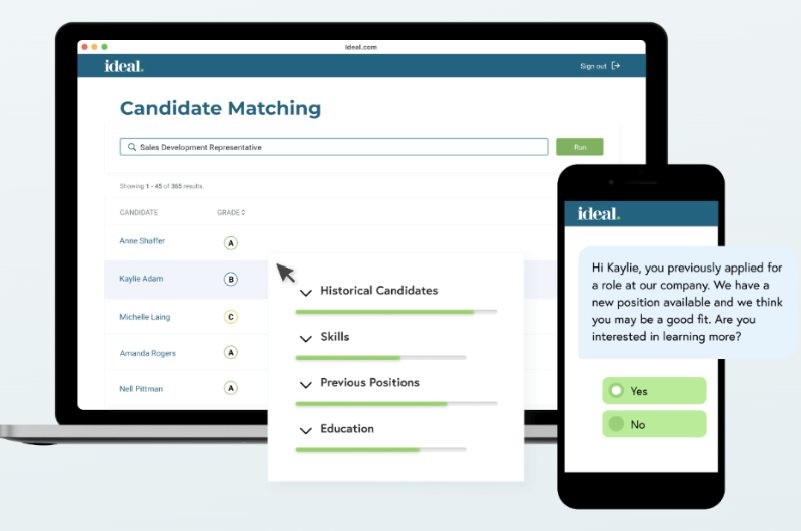
\includegraphics[width=5.46875in,height=\textheight]{ideal pic 1.png}

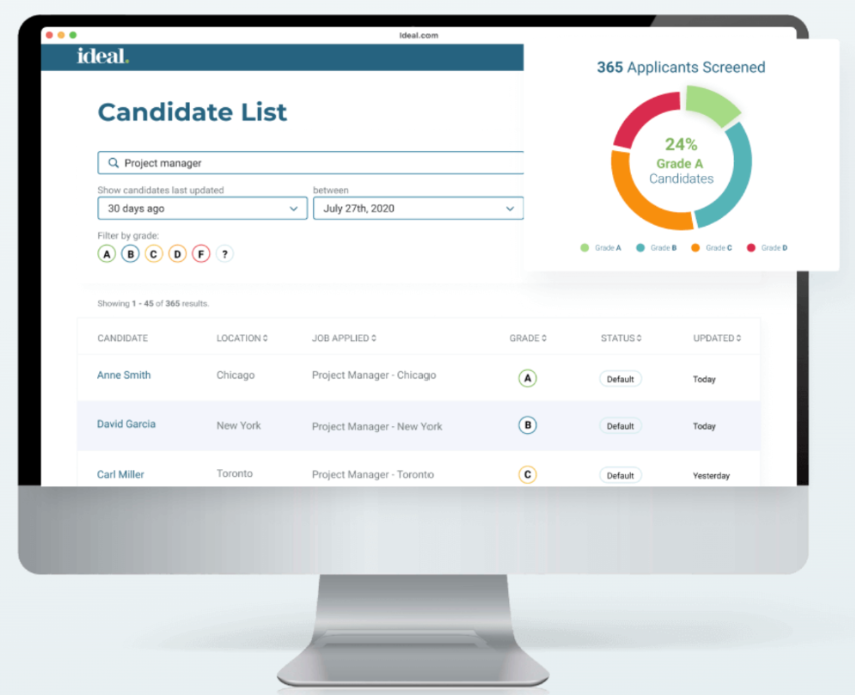
\includegraphics[width=3.57292in,height=\textheight]{ideal pic 2.png}

\hypertarget{hirevue}{%
\section{HireVue}\label{hirevue}}

\href{https://www.hirevue.com/}{HireVue} revolutionizes the hiring process through AI-driven tools, offering unparalleled flexibility and efficiency to both recruiters and candidates. With mobile-friendly, text-powered solutions, candidates can effortlessly schedule and partake in interviews anytime, anywhere, enhancing the overall experience. Recruiters benefit from the automation, which reduces time-intensive tasks like manual scheduling and candidate engagement.

The heart of HireVue is its commitment to fair and consistent hiring, relying on science-backed assessments rather than subjective instincts. Over \href{https://www.hirevue.com/our-science}{30 million interviews have informed HireVue's models}, emphasizing skills and behaviors over irrelevant details. The platform seamlessly integrates with existing ATS systems, eliminating time-consuming switches between platforms. Innovative features like HireVue Builder provide structured interviewing tools that standardize the interview process, ensuring fairer outcomes. Automated, conversational AI tools via SMS and Whatsapp streamline candidate interactions, making the process more engaging. With HireVue, the focus shifts from chasing candidates to efficiently and fairly hiring the best talent.

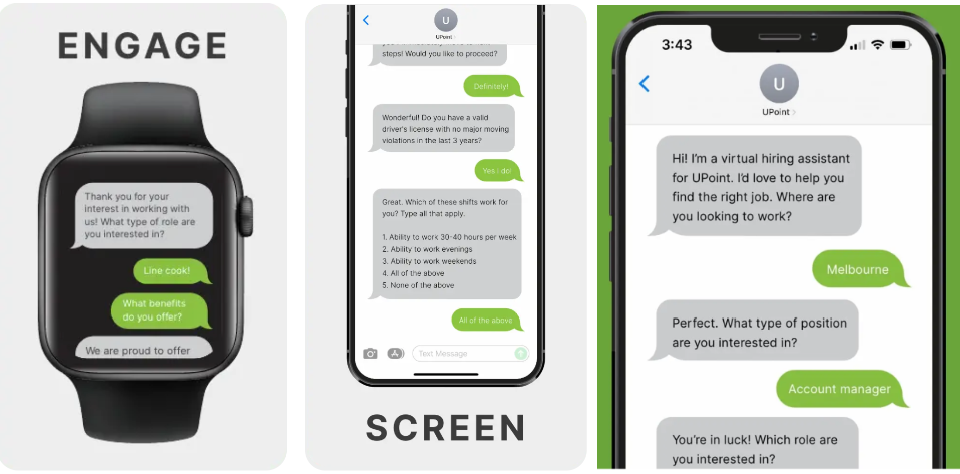
\includegraphics[width=5.57292in,height=\textheight]{hirevue pic.png}

\hypertarget{wade-wendy}{%
\section{Wade \& Wendy}\label{wade-wendy}}

\href{https://wadeandwendy.ai/}{Wade \& Wendy} revolutionizes talent acquisition by harnessing the power of AI, allowing recruiters to automate repetitive tasks and focus on enhancing the human touch in the recruitment process. Wendy facilitates 24/7 candidate engagement, parsing job descriptions to deliver personalized chats, and automating tasks from sourcing to scheduling, seamlessly integrating with existing recruitment systems. Meanwhile, Wade acts as a dynamic career guide for talent, personalizing job suggestions based on interactions. As the work landscape evolves with technology and shifting values, Wade \& Wendy ensure that recruiting remains human-centric, efficient, and adaptable, providing a symbiotic relationship between AI and human decision-making in the recruitment arena.

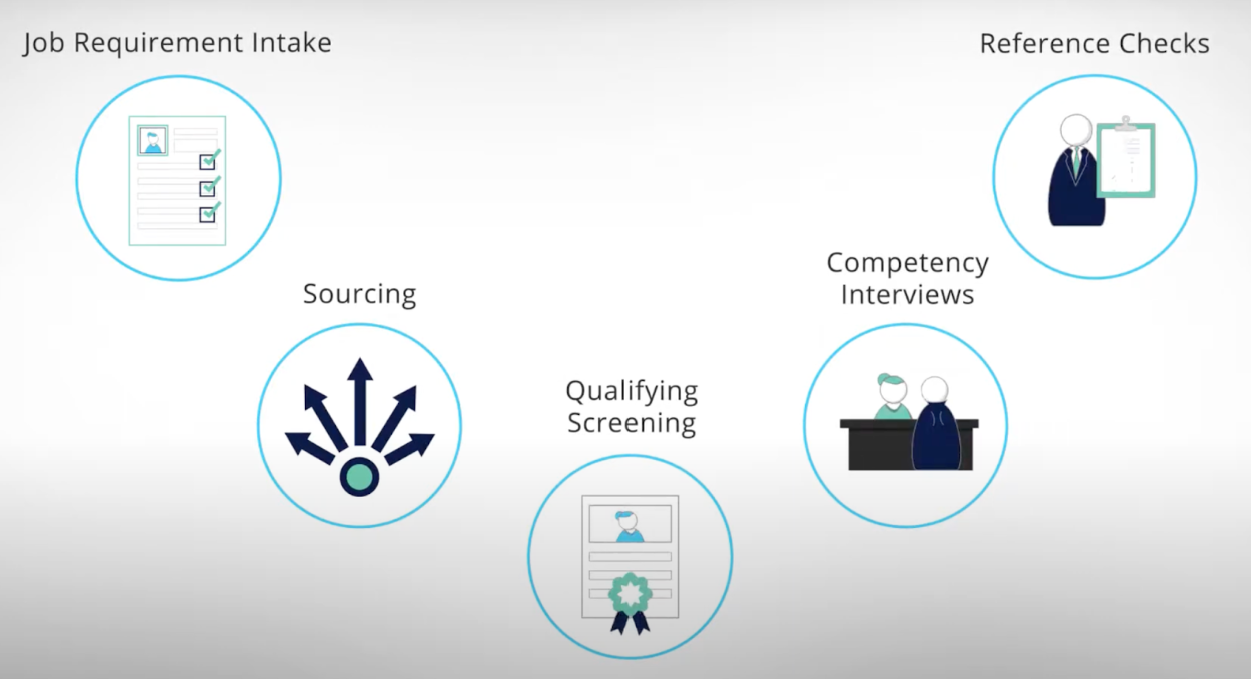
\includegraphics[width=5.45833in,height=\textheight]{wadewendy pic.png}

\hypertarget{what-you-a-student-can-do}{%
\section{What You (A Student) Can Do!}\label{what-you-a-student-can-do}}

For a student to successfully navigate and benefit from recruiting chatbots during their job search, they should consider the following strategies:

\begin{itemize}
\tightlist
\item
  \textbf{Familiarize with the common platforms and tools and algorithms} that companies use. This knowledge can help anticipate what to expect and how to interact with recruiting chatbots.
\end{itemize}

\begin{itemize}
\tightlist
\item
  When interacting with chatbots, \textbf{use clear language and be specific in your queries}. Avoid slang, abbreviations, or overly complex vocabulary since chatbots operate best with straightforward information.
\end{itemize}

\begin{itemize}
\tightlist
\item
  Chatbots are programmed to screen candidates based on predefined criteria. Anticipate and \textbf{prepare for standard questions} related to qualifications, experience, and job preferences.
\end{itemize}

\begin{itemize}
\tightlist
\item
  Make sure your \textbf{resume or online profile highlights your main qualifications, skills, and achievements} in a clear and organized manner. This helps the chatbot easily identify and match your profile with suitable roles.
\end{itemize}

\begin{itemize}
\tightlist
\item
  Given the 24/7 availability of chatbots, take advantage of this by \textbf{actively engaging with them}, asking questions, and seeking information about job roles, company culture, or application processes.
\end{itemize}

\begin{itemize}
\item
  If you feel the chatbot isn't adequately addressing your concerns or if you have specific questions, \textbf{ask for human intervention or look for alternative communication channels}.
\item
  While engaging with chatbots, \textbf{be wary of sharing overly personal or sensitive information} unless you're sure of the platform's privacy standards.
\end{itemize}

\begin{itemize}
\item
  Some advanced chatbots offer the option to \textbf{provide feedback}. Utilize this to clarify misunderstandings or to improve future interactions.
\item
  While chatbots are a valuable tool, \textbf{don't rely solely on them}. Use additional resources, such as career counselors, networking events, and traditional job platforms to complement your job search.
\end{itemize}

\hypertarget{resume-and-cover-letter-screening}{%
\chapter{Resume and Cover Letter Screening}\label{resume-and-cover-letter-screening}}

With the rise of AI tools and an increasing number of people graduating from college, job openings are experiencing large numbers of applicants. This is especially true for established companies that students want to work at because of their large societal impact and safer job security. For example, popular tech companies like Google, Apple, and Amazon and consulting firms like Deloitte, McKinsey \& Company, PwC, and EY have applicants from hundreds of colleges and universities and across the entire United States. To speed up the recruitment process, companies like these often use resume and cover letter screeners early on in their candidate selection process, so this chapter discusses how they use those tools and what students can do to better their chances.

\hypertarget{cvviz}{%
\section{CVViZ}\label{cvviz}}

\href{https://cvviz.com/product/resume-screening/}{CVViZ} is a groundbreaking AI tool designed to revolutionize resume screening for recruiters. Unlike conventional keyword searches, CVViZ employs contextual understanding to identify top candidates, learning from previous recruitment cycles to predict optimal matches. Its AI-driven approach eliminates the pitfalls of keyword mismatches, ensuring precise role differentiations. With CVViZ, recruiters can swiftly navigate through hundreds of resumes, leveraging its real-time relative ranking to pinpoint the best fits. Moreover, CVViZ seamlessly integrates with existing databases, enabling automated talent rediscovery for new job listings.~

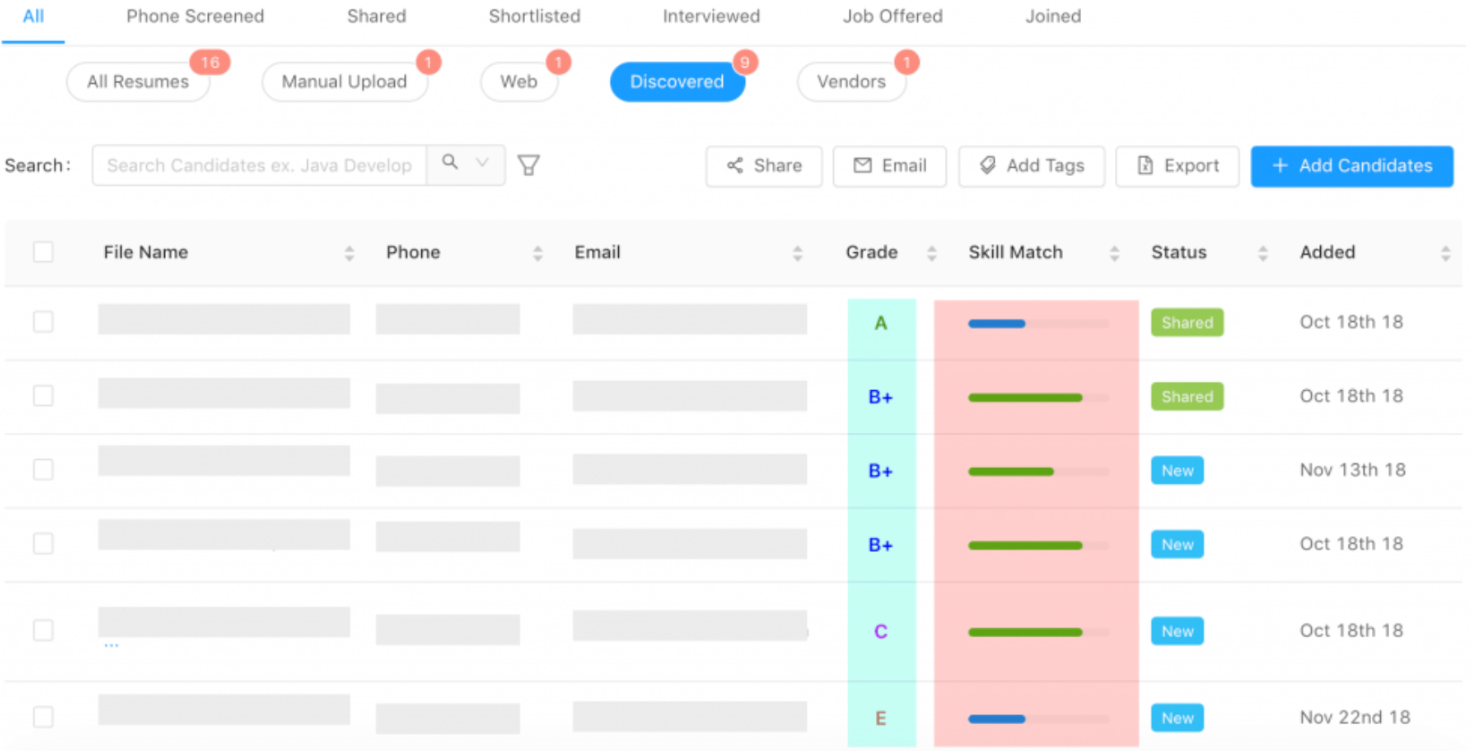
\includegraphics[width=5.44792in,height=\textheight]{cvviz pic 1.png}

The above picture shows the management dashboard for the recruiter to track candidates with their contact information, generated grade, skill match, and status. The below picture shows an example of how the tool identifies a specific keyword such as ``MySQL'' in candidates' resumes.

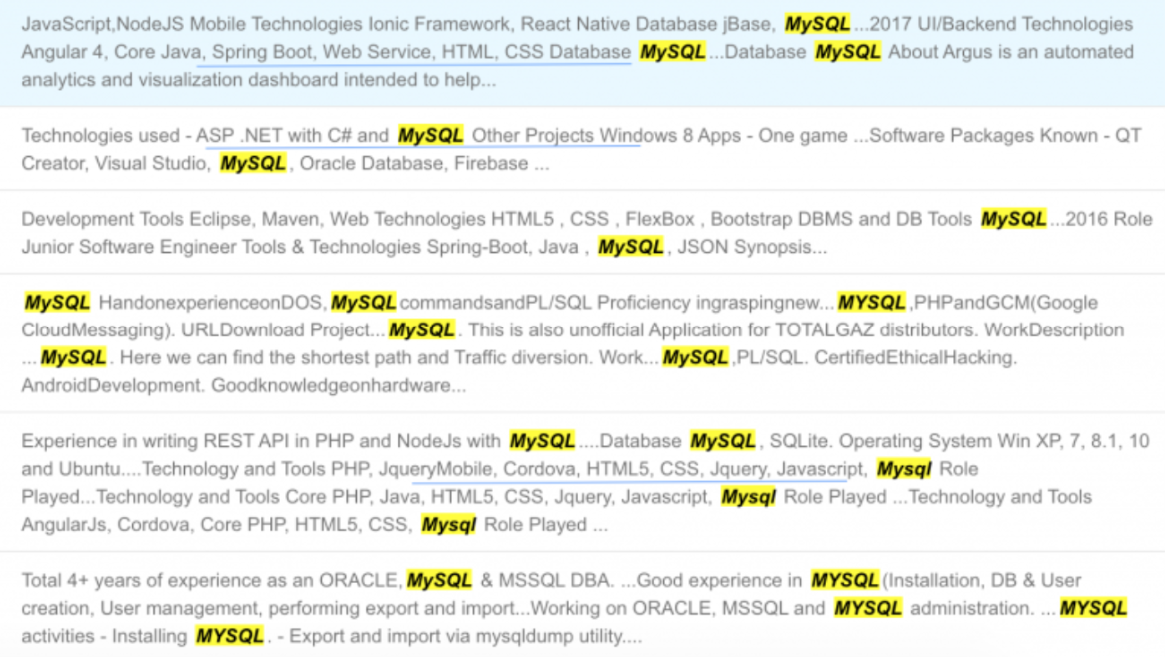
\includegraphics[width=5.36458in,height=\textheight]{cvviz pic 2.png}

\hypertarget{skeeled}{%
\section{Skeeled}\label{skeeled}}

\href{https://www.skeeled.com/services}{Skeeled} transcends traditional resume screening by seamlessly integrating a sophisticated ranking algorithm. This proprietary technology enables a refined and efficient candidate evaluation process, aligning qualification indicators with organizational requirements to present a meticulously curated shortlist.

Skeeled's remarkable utility extends further, catering to the bespoke demands of each enterprise. By accommodating customizable criteria such as specific driver's license categories, work permits, and other specialized prerequisites, Skeeled ensures a comprehensive assessment tailored to individual company prerequisites.

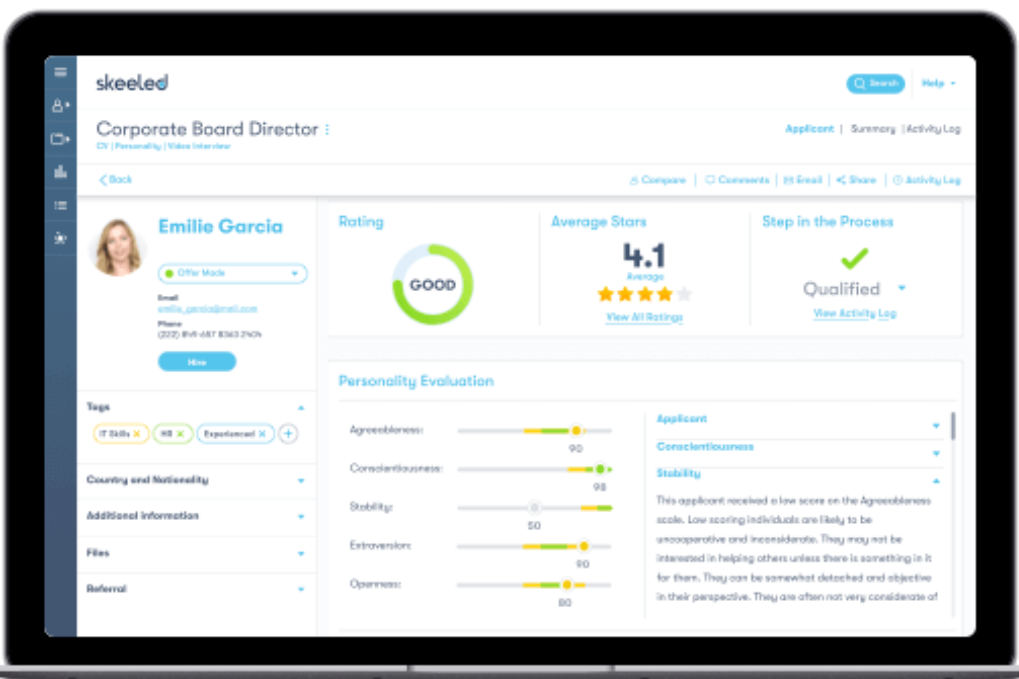
\includegraphics[width=5.30208in,height=\textheight]{skeeled pic.png}

\hypertarget{affinda}{%
\section{Affinda}\label{affinda}}

The standout feature of \href{https://www.affinda.com/resume-parser}{Affinda}'s offering is its advanced resume parser, powered by the robust AI engine known as Vega. One of the key advantages of Affinda lies in its adaptability. The machine learning algorithms underpinning the parser continually evolve, ensuring that it can cater to a wide array of recruitment scenarios, no matter how unique or specialized they may be. Unlike traditional parsers that rely on rigid keyword or grammar-based rules, Affinda harnesses the power of Natural Language Processing (NLP) to comprehend words and phrases in a manner akin to human understanding. This intuitive approach enhances the accuracy and relevance of parsed data, enabling recruiters to make more informed decisions.

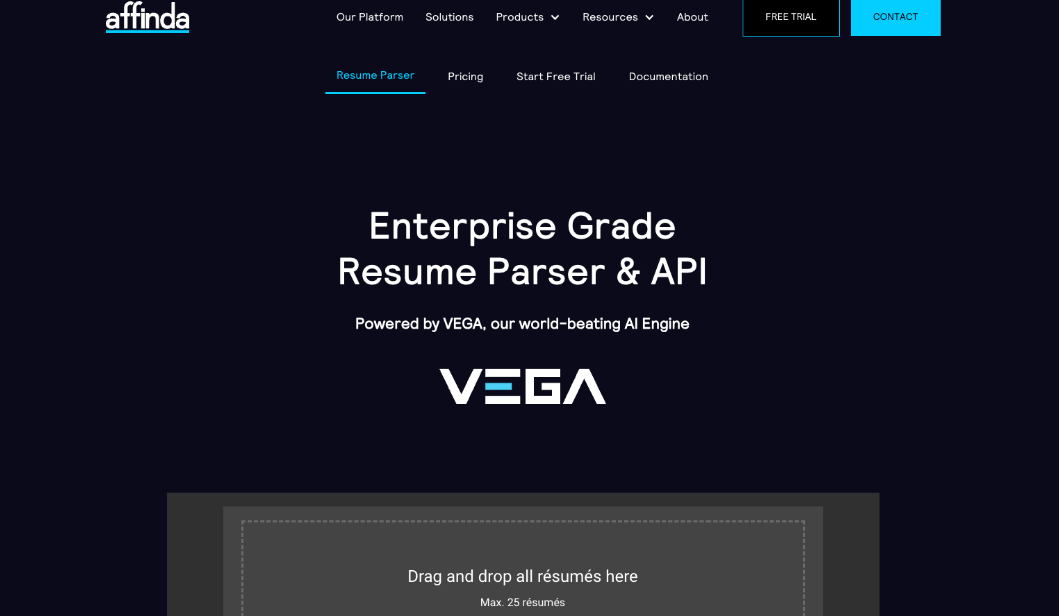
\includegraphics[width=3.9375in,height=\textheight]{affinda pic.png}

\hypertarget{what-you-a-student-can-do-1}{%
\section{What You (A Student) Can Do!}\label{what-you-a-student-can-do-1}}

Understanding what tools recruiters use to filter our candidates is the first step. By understanding the most popular tools, a few of which are referenced above, you can try to adjust your resume and cover letters to match what these tools search for and filter on. There are additional \href{https://www.indeed.com/career-advice/resumes-cover-letters/resume-ai\#:~:text=Instead\%20of\%20using\%20a\%20visual,this\%20kind\%20of\%20complex\%20information.}{recommended best practices} you can follow to ensure this step of the recruitment process is not where you fall out of the race with the company of your dreams:

\begin{itemize}
\item
  Triple check (or even quadruple check!) that there are \textbf{no typos or mispelled words}. It's much easier for an AI tool to discover these errors than a human
\item
  Use a \textbf{traditional, standard, and clean} resume format
\item
  Make sure to \textbf{submit the correct file type} for your resume (usually specified in the job application) as some AI tools can only process certain file types
\item
  Avoid using a visual resume, especially for technical roles. Opt for \textbf{plain text and relatively basic formatting}
\item
  Make a thorough attempt to \textbf{add keywords} to your resume that were mentioned in the job posting as the AI tool will look for these
\item
  Include a \textbf{mix of hard and soft skills} to showcase your diverse skill set
\item
  \textbf{Traditional or usual resume advice still applies} to the resumes you submit to be analyzed by AI tools
\end{itemize}

\hypertarget{video-interview-assessments}{%
\chapter{Video Interview Assessments}\label{video-interview-assessments}}

One way that recruiters may also quicken the recruitment process is to use AI tools that analyze video interviews, whether self-recorded by the candidate or from an actual interview with employees from the company. More commonly, though, the video interview assessment that an AI conducts will be through a self-recorded interview the candidate will record on the employer's hiring platform. \textbf{Watch the following video for a concise summary of how AI can be used in the interview process!}

\href{https://www.youtube.com/watch?v=cJkHft032OE}{The AI Video Interview}

\hypertarget{how-it-works}{%
\section{How it Works}\label{how-it-works}}

It's important to note that the extent or amount of influence an AI tool will have will vary on the company. One company may not use AI tools at all to analyze a recorded interview video, whereas another company may use AI as a supplemental analysis to support decision making or just rely entirely on AI to filter out candidates.

In general, a video interview assessment entails a question being shown to the candidate, and then a brief period, usually around 30 seconds, for the candidate to prepare and formulate a response. Then, the tool will record the candidate's response (video and audio) for the allotted time for that question, which is usually just a few minutes. There may be an option to redo the video one time without a penalty, but don't rely on it as that is not always an option. Afterwards, the AI tool will create a report based on two main elements: \textbf{facial analysis} and \textbf{language analysis} (1).~

\hypertarget{facial-analysis}{%
\subsection{Facial Analysis}\label{facial-analysis}}

Facial analysis will focus on the non-verbal aspect of the interview or how you conduct yourself during the recordings. This may include things such as \textbf{eye contact} with the camera, \textbf{eye wandering}, \textbf{lip position} and \textbf{movements}, \textbf{eyebrow movements} (furrowing and raising), \textbf{amount of smiling}, \textbf{chin raising}, and more (2).


\includegraphics[width=3.46875in,height=\textheight]{Facial_Analysis.png}

\hypertarget{language-analysis}{%
\subsection{Language Analysis}\label{language-analysis}}

On the other hand, language analysis will focus on the content of your responses and the nature of your delivery. During or immediately after the recorded interview, the AI tool will convert your responses to text. Then, it'll parse through this and look for various things. From a content perspective, this may include the \textbf{technical language} and \textbf{vocabulary} you use that aligns with the job description and what the company is looking for (1). From a delivery perspective, this may include \textbf{active vs passive voice}, \textbf{run-on sentences}, the use of \textbf{filler words}, and the \textbf{tone} of your voice.

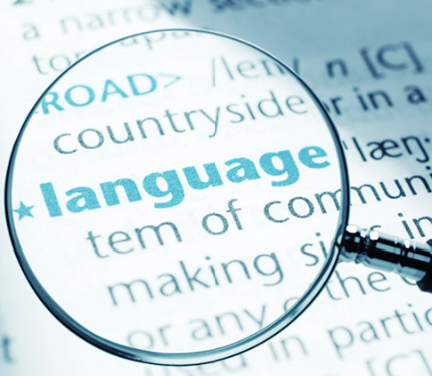
\includegraphics[width=2.16667in,height=\textheight]{Language_Analysis.png}

\hypertarget{benefits-1}{%
\section{Benefits}\label{benefits-1}}

AI-assessed interviews provide numerous benefits for both the recruiter and candidate:

\begin{itemize}
\item
  \textbf{Recruiters}

  \begin{itemize}
  \item
    Allows the company to accept more applicants to the open position~
  \item
    Spend less money on employees to assess the video recordings
  \item
    Removes the bottleneck of screening the recordings by hand
  \end{itemize}
\item
  \textbf{Candidates}

  \begin{itemize}
  \item
    While there is always a deadline, you can choose to do the recorded interview when it works best in your schedule
  \item
    More fair hiring process that isn't influenced as much by preconceptions and human biases and instead focuses more on qualifications
  \end{itemize}
\end{itemize}

\hypertarget{drawbacks}{%
\section{Drawbacks}\label{drawbacks}}

While AI-assessed interviews have its benefits, there are some significant drawbacks:

\begin{itemize}
\item
  AI tools must be coded by humans in the first place, so there is no guarantee that the tool will be free of human biases
\item
  They may reinforce discriminatory practices such as penalizing someone with a strong accent or speed impediment
\item
  Human emotions and facial expressions are very complex and may not be interpreted correctly, which can inadvertently remove a qualified candidate from the selection process
\item
  Concerns regarding personal privacy and data security due to the large amounts of information being collected during the recordings
\end{itemize}

\hypertarget{what-you-a-student-can-do-2}{%
\section{What You (A Student) Can Do!}\label{what-you-a-student-can-do-2}}

As a student preparing for the recruiting process this upcoming school year, you may be wondering how you can best set yourself up for success if you ever experience one of these AI interviews. \textbf{Look no further!} The following subsections highlight some tips and best practices.

\hypertarget{general-preparation}{%
\subsection{General Preparation}\label{general-preparation}}

General preparation relates to activities and preparation work you should be doing prior to the interview to ensure you're best prepared to answer the questions.

\begin{itemize}
\item
  Research the company and general job type thoroughly in case of any questions related to why you want to work for the company or why you are applying to that positions
\item
  Prepare what you are going to say. Research some \href{https://www.themuse.com/advice/interview-questions-and-answers}{commonly asked interview questions} and make sure you have a story bank of your past experiences that you can pull from and adjust based on the question asked
\item
  Practice using the \href{https://www.themuse.com/advice/star-interview-method}{STAR (situation, task, action, result) method} as it's very popular framework for providing a response that is coherent, comprehensive, and insightful
\end{itemize}

\hypertarget{countering-the-ai-tools}{%
\subsection{Countering the AI Tools}\label{countering-the-ai-tools}}

Countering the AI tools relates to what you should do during the interview based on what the AI tools are looking for and analyzing.

\begin{itemize}
\item
  \textbf{Practice talking to a camera and recording yourself} so you get a good feel for where you're at and how to make progress (see Chapter 6: Student Practice Interviews)
\item
  \textbf{Dress nice} as if you were being interviewed by an actual interviewer in person
\item
  \textbf{Clean the background of your recording space} so the AI tool doesn't penalize you for a distracting background or make it harder for it to more accurately read your facial expressions
\item
  Ensure your \textbf{lighting is good} to allow for a proper facial analysis by the AI
\item
  Try to \textbf{maintain eye contact with the camera} as much as possible and use sticky notes on the computer/laptop if you want to refer to material
\item
  Keep your \textbf{head high or at a neutral position}; avoid angling your head downward
\item
  \textbf{Smile} and maintain a happy facial expression
\item
  \textbf{Avoid} the use of filler words like \textbf{``um'', ``like'', or ``hmm''}
\item
  Use \textbf{keywords} (skills and job duties) from the job description during your responses if you can
\item
  \textbf{Speak clearly and loudly} (more than usual) to ensure the AI tool can translate your verbal response into text
\item
  \textbf{Try not to furrow your eyebrow}s as it can be interpreted as confusion, disapproval, or worry
\end{itemize}

\hypertarget{skill-assessments}{%
\chapter{Skill Assessments}\label{skill-assessments}}

In today's dynamic job market, where diverse candidate profiles are the norm, there's a pressing need for robust and accurate recruitment measures. Skill assessments, as a result, have emerged as an essential tool, allowing companies to authenticate abilities and promote a hiring process grounded in merit and transparency. At the forefront of this evolution is the incorporation of artificial intelligence (AI) into assessment techniques. AI-driven assessment tools, enhanced by machine learning capabilities, are reshaping the way organizations approach recruitment. Through these tools, enterprises can not only pinpoint top talent but also delve deeper into their competencies beyond what traditional resumes reveal (1). Below is an in-depth analysis of some of the innovative AI-powered assessment tools that are redefining recruitment standards (2).

\hypertarget{devskiller}{%
\section{DevSkiller}\label{devskiller}}

\href{https://devskiller.com/}{DevSkiller} offers a sophisticated solution tailored to the needs of technical recruitment. With over \href{https://devskiller.com/talentscore/}{5,000 pre-set tasks} that closely mirror real-world challenges, it ensures thorough evaluations of candidates across various technical areas such as front-end, back-end, mobile, DevOps, and security.

Prioritizing a genuine testing environment, DevSkiller allows candidates to work within their usual development settings and engage in CI/CD processes based on Git repositories. This approach evaluates more than just coding skills---it delves into a candidate's expertise with specific libraries, frameworks, tools, and databases.

The platform's ``CodePair with video'' feature enhances the evaluation process by enabling remote interviews. This way, recruiters can directly observe a candidate's problem-solving approach and thinking process. For organizational ease, DevSkiller integrates smoothly with Applicant Tracking Systems (ATS) and offers customization options for branding. Its advanced reporting tools assist recruiters in making well-informed decisions. Whether using the platform's standard tests or tailoring assessments to specific roles, DevSkiller proves to be a valuable tool for tech recruitment.

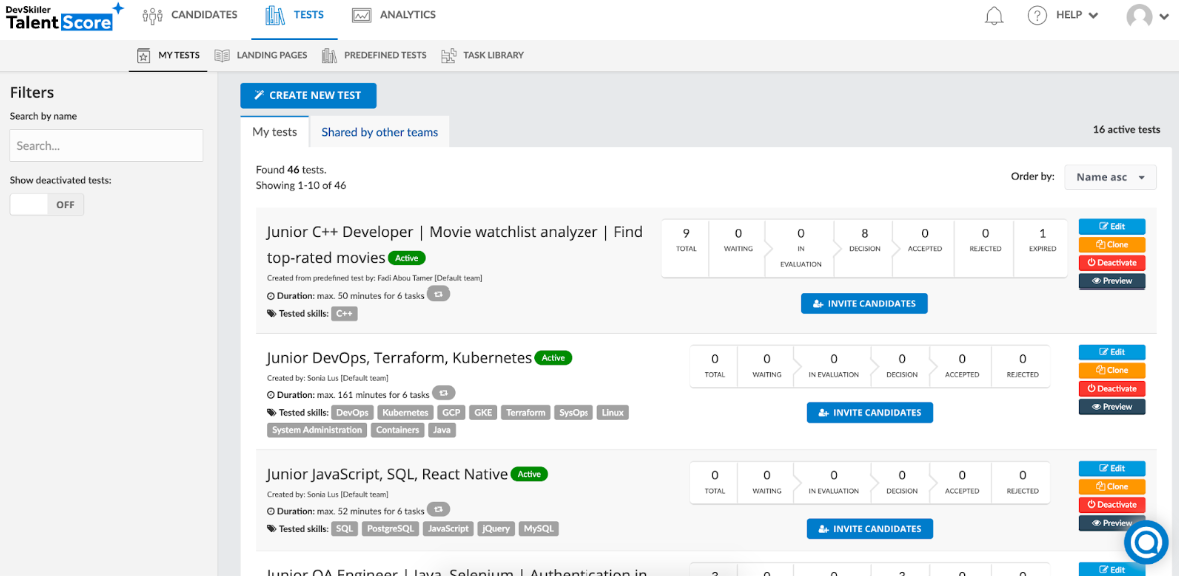
\includegraphics[width=4.73958in,height=\textheight]{devskiller picc.png}

\hypertarget{testgorilla}{%
\section{TestGorilla}\label{testgorilla}}

\href{https://www.testgorilla.com/?utm_term=testgorilla\&utm_campaign=TestGorilla+\%7C+Branded+I+SKAG+AdGroups+\%7C+US\&utm_source=google\&utm_medium=cpc\&hsa_acc=4932434860\&hsa_cam=12598017525\&hsa_grp=118410898783\&hsa_ad=537212466646\&hsa_src=g\&hsa_tgt=kwd-927907651583\&hsa_kw=testgorilla\&hsa_mt=e\&hsa_net=adwords\&hsa_ver=3\&gclid=CjwKCAjw5_GmBhBIEiwA5QSMxLAMrdiiKyGt8ZjFz4BL_vP1ktTPpNCugXM2c48T20vqlbD_7lhF1hoCWDEQAvD_BwE}{TestGorilla} revolutionizes the recruitment process, making the traditional reliance on CVs obsolete. Instead of sifting through piles of resumes, this platform offers talent assessments that pinpoint the most suitable candidates, making the hiring process quicker, streamlined, and devoid of biases. By utilizing a library of \href{https://www.testgorilla.com/?utm_term=testgorilla\&utm_campaign=TestGorilla+\%7C+Branded+I+SKAG+AdGroups+\%7C+US\&utm_source=google\&utm_medium=cpc\&hsa_acc=4932434860\&hsa_cam=12598017525\&hsa_grp=118410898783\&hsa_ad=537212466646\&hsa_src=g\&hsa_tgt=kwd-927907651583\&hsa_kw=testgorilla\&hsa_mt=e\&hsa_net=adwords\&hsa_ver=3\&gclid=CjwKCAjw5_GmBhBIEiwA5QSMxLAMrdiiKyGt8ZjFz4BL_vP1ktTPpNCugXM2c48T20vqlbD_7lhF1hoCWDEQAvD_BwE}{358 scientifically-backed tests}, TestGorilla provides predictions on real-world job performance, assessing both job-specific skills such as coding and broader competencies like critical thinking.

Beyond skill assessments, the platform's unique personality and value tests offer a holistic view of candidates, treating them as individuals rather than mere profiles on paper. This results in a more efficient recruitment process where screening CVs and preliminary interviews become redundant. The automated grading system ranks candidates, enabling recruiters to view video responses and evaluate potential hires in a fraction of the usual time.

Moreover, TestGorilla champions diversity and equal opportunity. The platform ensures that all candidates receive a fair chance, thus promoting diverse team compositions which are known to enhance performance. In the pursuit of offering a gratifying experience, the platform's professionally crafted tests act as an extension of the company's branding, engaging and motivating candidates to put their best foot forward.

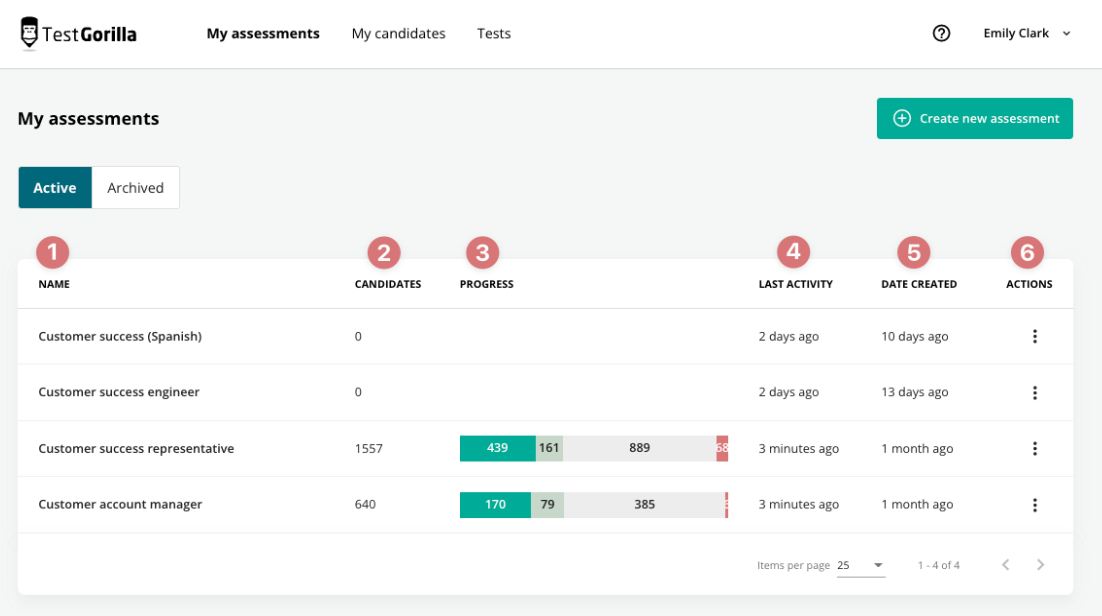
\includegraphics[width=4.35417in,height=\textheight]{testgorilla pic.png}

\hypertarget{pymetrics}{%
\section{Pymetrics}\label{pymetrics}}

\href{https://www.pymetrics.ai/}{Pymetrics} champions a transformative approach to talent assessment, placing potential over traditional qualifications. Using gamified assessments, the platform objectively evaluates cognitive and behavioral traits, offering insights beyond conventional resumes.

Tailoring its approach, Pymetrics crafts bespoke talent algorithms for each company, ensuring alignment with unique definitions of top talent. This customization not only streamlines hiring but also bolsters engagement, mobility, and retention. Regular bias-checks on these algorithms reaffirm the platform's commitment to ethical talent acquisition.

Instead of rejecting, Pymetrics focuses on redirecting candidates, ensuring everyone finds their niche. The platform's ``Core Games'' swiftly assess numerical and logical reasoning, while its suite of patented games paints a detailed behavioral profile in less than 30 minutes (3).

Integrated digital interviews enrich the assessment process, with role-specific questions ensuring unbiased evaluations. Recruiters benefit from collaborative features, like shareable videos, while candidates enjoy a flexible interview experience with practice and re-recording options.

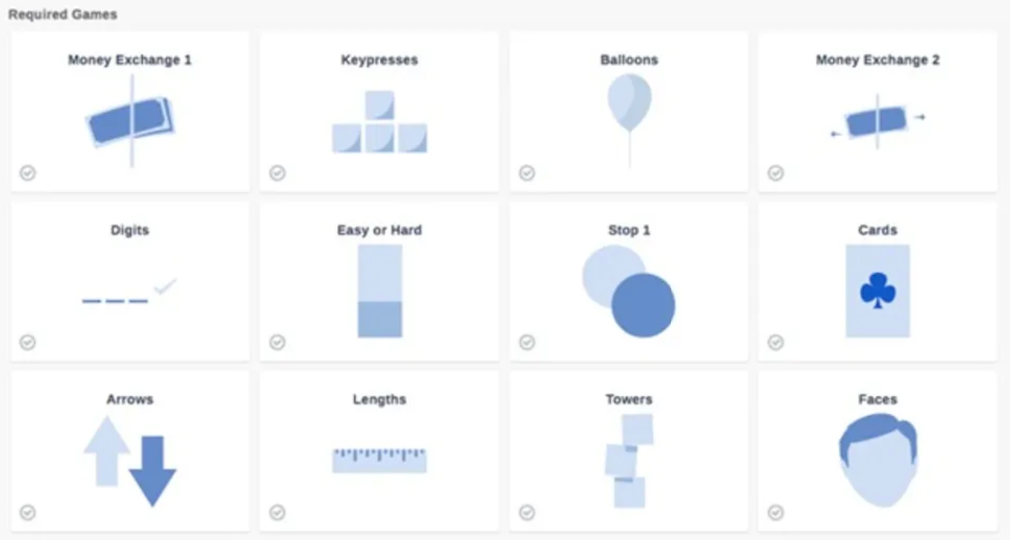
\includegraphics[width=4.75in,height=\textheight]{pymetrics pic2.png}

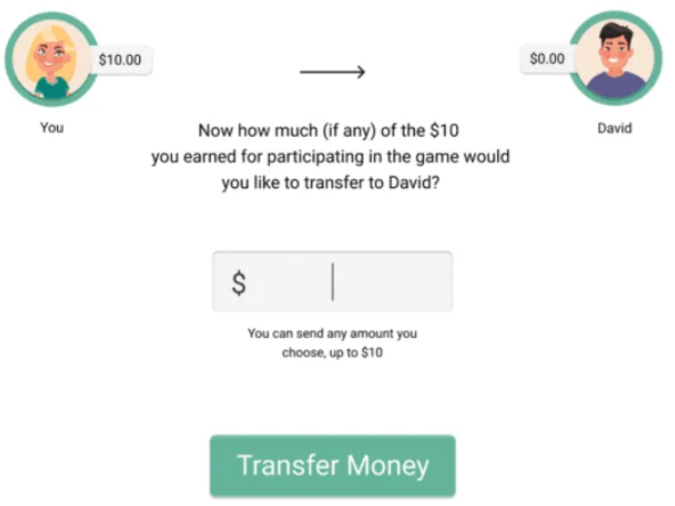
\includegraphics[width=3.78125in,height=\textheight]{pymetrics pic1.png}

Boston Consulting Group (BCG), a well-established management consulting firm that is often the target of University of Michigan students, uses Pymetrics in their candidate recruiting process. To see how BCG uses it, please refer to the following link: \url{https://mconsultingprep.com/bcg-pymetrics-test}

\hypertarget{what-you-a-student-can-do-3}{%
\section{What You (A Student) Can Do!}\label{what-you-a-student-can-do-3}}

There is only so much preparation and practice you as a student can do to maximize your success on these skill assessments. A few intuitive tips and best practices can be found below:

\begin{itemize}
\item
  \textbf{Get quality sleep} before doing skill assessments
\item
  \textbf{Practice} commonly required skills
\item
  \textbf{Touch up on skills} mentioned in the job listing
\item
  \textbf{Be honest} while completing the assessments
\end{itemize}

\hypertarget{predicting-candidates-success}{%
\chapter{Predicting Candidates' Success}\label{predicting-candidates-success}}

While the ideal job position is a two-way street in which the candidate wants the company and the company wants the candidate, ultimately, the company wants to know how you will perform and help it improve its overall performance. One way to do this is to use AI tools that can predict the success you may have in the role and how you conduct yourself. The following subsections describe exactly what this is and how it works.


\includegraphics[width=3.23958in,height=\textheight]{predict success.jpg}

\hypertarget{personality-and-trait-assessments}{%
\section{Personality and Trait Assessments}\label{personality-and-trait-assessments}}

One way that recruiters may predict candidates' success in a role is by better understanding their personality traits. Recruiters can now leverage AI tools to assess these personality traits. Ultimately, they want to know how you may interact with other people and what you may do in various situations.

\hypertarget{zelfium}{%
\subsection{Zelfium}\label{zelfium}}

\href{https://www.zelfium.com/\#/}{Zelfium} distills 300+ scientifically verified personality factors into 7 major traits, 14 sub-traits, and 36 components using machine learning, particularly neural deep networks. Zelfium's innovation lies in its use of AI to analyze user responses and behaviors, resulting in a highly accurate personality profile. This dynamic process continuously refines results, offering a comprehensive understanding of human personalities worldwide.

\hypertarget{predictive-models-for-roles}{%
\section{Predictive Models for Roles}\label{predictive-models-for-roles}}

Organizations can leverage their historical data to build predictive models for specific roles, which are often trained by AI algorithms that pull from previous or current employees at the company who have been successful. This can then be used in assessing potential candidates in the future.

\hypertarget{affinix}{%
\subsection{Affinix}\label{affinix}}

\href{https://www.peoplescout.com/technology/}{Affinix} by PeopleScout is an innovative AI sourcing tool driven by predictive analytics technology. It assists employers in identifying success-predicting qualities and swiftly locating candidates who align with these traits across various platforms. The tool's predictive capabilities improve over time as recruiters input more data, culminating in refined candidate predictions. This ensures that AffinixTM maximizes its predictive analytics potential and enhances the efficiency of talent acquisition.

\hypertarget{behavior-analysis}{%
\section{Behavior Analysis}\label{behavior-analysis}}

Similar to personality and trait assessments, companies may use AI tools to predict the behavior of candidates in a working environment and how that may impact their ability to succeed in a specific role.

\hypertarget{the-pi-behavioral-assessment}{%
\subsection{The PI Behavioral Assessment}\label{the-pi-behavioral-assessment}}

\href{https://www.predictiveindex.com/assessments/behavioral-assessment/?creative=655858294556\&keyword=predictive\%20personality\%20test\&matchtype=b\&network=g\&device=c\&utm_source=google\&utm_medium=ppc\&utm_content=bofu-brand-low-value\&device=c\&matchtype=b\&utm_term=predictive\%20personality\%20test\&gad=1\&gclid=Cj0KCQjwldKmBhCCARIsAP-0rfw2xB87svR2BFTESJ6nSMzDqIs8ni8VKXiD1robOSabO6uU7wTWjagaAoHUEALw_wcB}{The PI Behavioral Assessment} is an advanced AI tool that goes beyond traditional personality tests. It quickly uncovers an individual's natural behavioral drives and needs, helping predict their actions in various situations. By answering two questions about expected work behavior and self-perceived behavior, participants are assigned one of 17 Reference Profiles, offering insights into their innate tendencies. The assessment measures four key behavioral drives: dominance, which influences control; extroversion, driving social interaction; patience, seeking stability; and formality, promoting rule conformity. This tool empowers organizations to make informed hiring and team-building decisions, enhancing workplace dynamics and performance.

\hypertarget{what-you-a-student-can-do-4}{%
\section{What You (A Student) Can Do!}\label{what-you-a-student-can-do-4}}

\begin{itemize}
\item
  Use assessment results to \textbf{pinpoint areas for improvement}, and dedicate time to refine these skills and behaviors through online courses, workshops, and self-study. Strengthening your abilities will position you as a competitive candidate in job applications and promotions
\item
  Leverage behavioral assessments and personality questionnaires to \textbf{gain deeper insights into your strengths, weaknesses, and behavioral traits}. Armed with this self-awareness, tailor your career path to match your attributes and work on any areas that could be holding you back
\item
  Tap into predictive analytics tools to \textbf{stay attuned to shifting job market trends} and the skills in demand. Use this foresight to adjust your educational path, ensuring it aligns with these trends. If you're already employed, identify opportunities for upskilling or reskilling to remain valuable in your role or when pursuing new avenues
\item
  Take your time when completing these and \textbf{answer questions thoughtfully}. You want recruiters to have an accurate representation of who you are as a person and how you can contribute to their company
\end{itemize}

\hypertarget{conclusion}{%
\chapter{Conclusion}\label{conclusion}}

As you have just taken a journey through our website, it is evident that AI is playing an increasingly important role in the entire recruitment process from both perspectives: the candidate and employer. Through discussing tools Ross students can use in the application process and also detailing how recruiters are using AI tools, we hope we have provided you with a comprehensive website you can refer to in the coming months.~

Best of luck to you in securing your dream job!!!


\includegraphics[width=4.41667in,height=\textheight]{conclusion pic.png}

\hypertarget{our-working-process}{%
\chapter{Our Working Process}\label{our-working-process}}

\hypertarget{mid-point-check-in-survey}{%
\section{Mid-Point Check-In Survey}\label{mid-point-check-in-survey}}

Only 4/5 of our team members completed the mid-point check-in survey, but we obtained the remaining team member's feedback at a later date. The majority of the anonymous feedback was very positive. There was a 1 out of 5 rating for "Listening" but this was just a mistake one team member made when filling out their survey. Every category was ranked at least a 3 out of 5, with a majority of them being a 4 or 5. It seemed everybody has happy with the direction of our team and project outputs so far.~

\textbf{What is one thing we have been doing really well as a team?}

Our responses to this question were underscored by the following themes: time management and supportiveness. Whenever we met as a team, the meetings were always productive and everybody had a clear idea of what the purpose of the meeting was and what work we should be completing inbetween meetings.

\textbf{What is one thing we should do differently as a team moving forward?}

There were a few areas for improvement that team members highlighted. These were increasing our communication during the last few weeks of the semester as there was a lot of work due and conducting performance reviews for improvement and getting feedback. We tried to improve upon these things after we received the survey results, and we were mostly satisfied with the results.

\hypertarget{meeting-strategy}{%
\section{Meeting Strategy}\label{meeting-strategy}}

Our meeting strategy for the project was designed to optimize our collaboration and ensure consistent progress toward our goals. We structured our meetings to provide a balanced blend of virtual and in-person interactions. By meeting 2-3 times a week, we ensured consistent communication and alignment among team members. Our Zoom meetings serve as dynamic platforms for discussing coding strategies, brainstorming solutions, and addressing technical challenges. In contrast, our in-person meetings are dedicated to refining our presentation materials, enhancing our communication skills, and polishing our project deliverables. Additionally, our regular check-in meetings provided opportunities for quick updates, progress tracking, and issue resolution, further fostering a efficient teamwork environment.

\hypertarget{communication-strategy}{%
\section{Communication Strategy}\label{communication-strategy}}

Our team followed a seamless and efficient communication strategy. We chose GroupMe as our primary platform for active communication, ensuring instant updates, quick clarifications, and the ability to share important announcements. In addition, we utilized email threads to coordinate and schedule study room sessions, enabling us to optimize our study and work sessions effectively. Our shared Google Doc served as a centralized hub for managing all project content, allowing us to collaboratively contribute, edit, and organize our work. The feature of adding comments on each others' work within the shared Google Doc ensured constructive feedback and promoted a culture of continuous improvement among our team members.

\hypertarget{navigating-conflict}{%
\section{Navigating Conflict}\label{navigating-conflict}}

Our group truly showed the essence of teamwork. Whenever we encountered obstacles that left us in a bind, our collective response was to regroup, huddle up, and carefully reconsider our approach. The synergy within our team was such that conflicts hardly arose; however, even in those rare instances, our ability to swiftly reconcile differences was impressive. This collaboration and quick conflict resolution not only kept us on track but also nurtured an environment where collaboration and psychological safety thrived. Our shared commitment to open communication and mutual respect allowed us to navigate challenges with a common goal and allowed us to view the bigger picture, ultimately leading to a great number of successful outcomes. We also dedicated time after presentations and submitting project deliverables to reflect on our success and areas for improvement. This commitment to honesty also helped us mitigate and minimize conflict.

\hypertarget{managing-bookdown-and-github}{%
\section{Managing Bookdown and GitHub}\label{managing-bookdown-and-github}}

Going into this project, none of us had any significant experience with GitHub nor Bookdown. However, a few members of our team had prior experience with R and RStudio. Michael invested time early in the project to set up the GitHub repository and the GitHub Pages website. Team members individually set up their RStudio and downloaded the required packages and installs to be able to push and pull to GitHub. We had a few impromptu meetings to ensure everybody\textquotesingle s technology was working smoothly and there were no significant issues. During this troubleshooting stage, we relied on each other and Google to gather information and knowledge to debug issues we ran into. Additionally, we also documented the steps and procedures to properly commit, push, pull, and build the book. Overall, while we came into this project with minimal experience in this area, our commitment to learning and using each other as a resource proved to be invaluable to our ability to build a respectable website.

\hypertarget{how-we-were-agile}{%
\section{How We Were Agile}\label{how-we-were-agile}}

Our team embraced the Agile methodology as the basis of our working process. As the Agile Manifesto highlights, we value "Responding to chage over following a plan."~ We broke our project into small sections and focused on specific sections at a time, building upon them and working in increments.~

We also valued "Individuals and interactions over processes and tools\textquotesingle\textquotesingle{} mentioned in the Agile Manifesto. Our team had excellent collaboration, where team members help each other when challenges arise, work together on tasks and overcome challenges, and leverage each member\textquotesingle s expertise.

In addition, we translated Agile\textquotesingle s "Working solutions over comprehensive documentation" into our team approach to meetings and communication. We held a mix of in-person and virtual meetings based on the amount of meeting preparation work and the type of work to be done in the meetings to maximize working productivity and efficiency.

By efficiently and successfully breaking work into increments, embracing collaboration, and adapting various communication methods, we built a team environment that strongly aligned wth the Agile Manifesto\textquotesingle s values, which helped us achieve project success.

Additionally, we ensured everybody had a clear understanding of their roles and responsibilities, and we made sure everyone else was aware of each others' responsibilities too. For example, we had a Google Doc that we used to build and craft the majority of our content for the website. We delegated sections of the website to be completed by each team member, and we carefully tracked and monitored everybody\textquotesingle s status as seen below. This helped our team adapt to change and assist other team members very easily and efficiently when those moments arose.

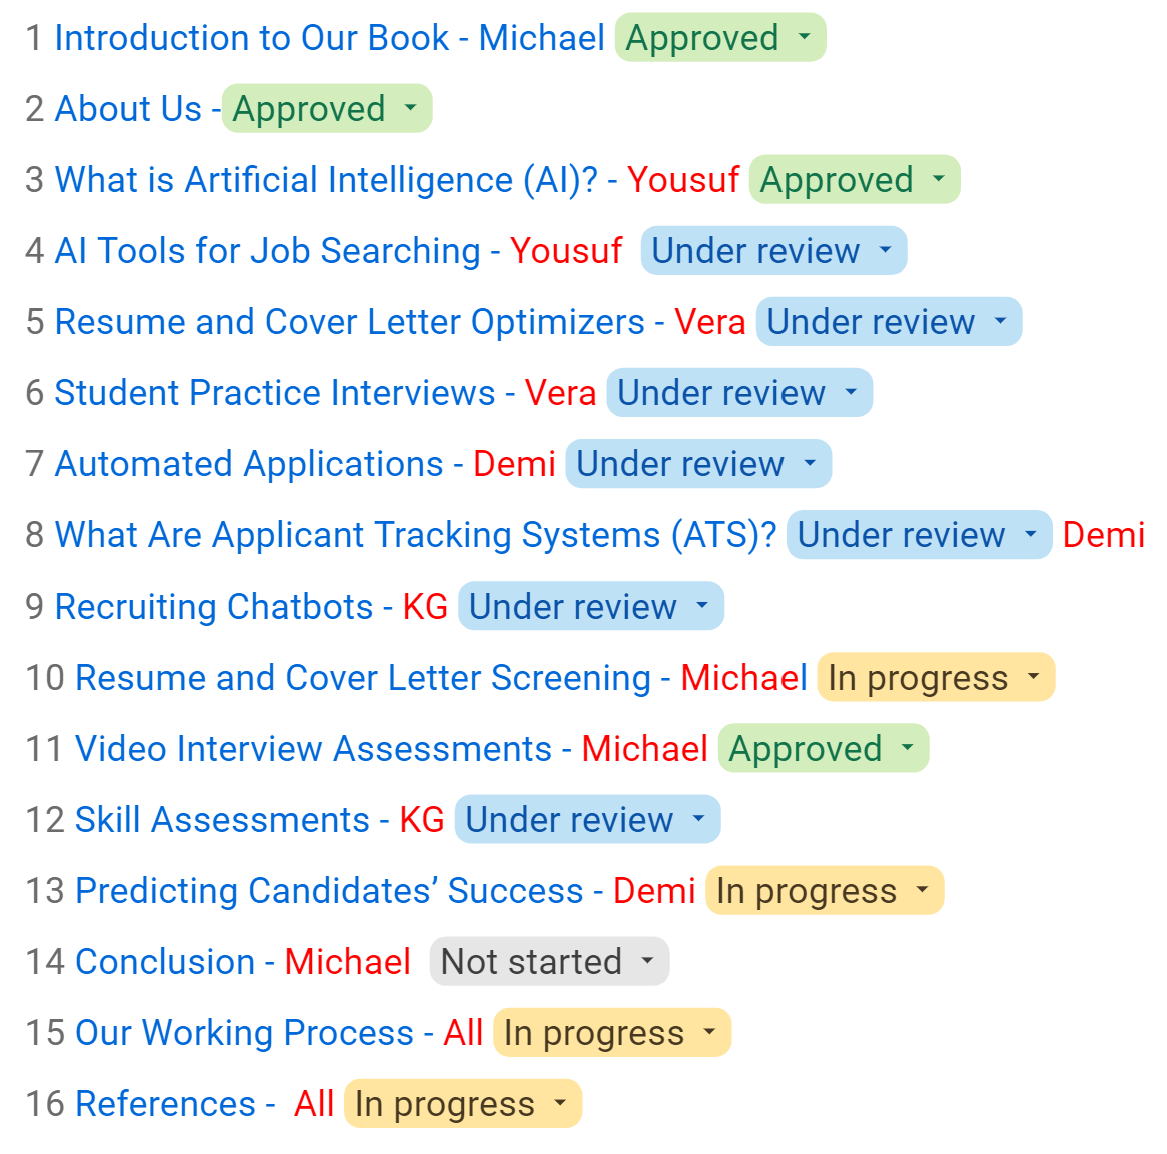
\includegraphics[width=5.52083in,height=\textheight]{work delegation.png}

\hypertarget{fostering-psychological-safety}{%
\section{Fostering Psychological Safety}\label{fostering-psychological-safety}}

Over the summer, our team's cohesion has been underscored by a deep-rooted psychological safety. From the outset, we prioritized an environment of trust and open communication, ensuring that every member felt both comfortable and empowered. This was not just evidenced in the absence of concerns regarding comfort, but also in the equal weight given to each voice and idea. Whether voicing differing opinions, addressing concerns, or delivering challenging news, the team always met each other with understanding rather than judgment. It's worth noting that our team culture was not one of mere tolerance, but active acceptance. Mistakes, instead of becoming points of contention, were treated as opportunities for growth. Every team member could confidently rely on their peers for help, knowing well that their efforts would never be intentionally sabotaged. For example, Demi was very open to helping out other team members complete their sections as she had completed her individual section work pretty quickly. Furthermore, what truly set our group apart was the recognition and harnessing of individual strengths. Each person's unique talents and skills were celebrated and utilized, elevating the overall quality of our collaborative projects.

\hypertarget{references}{%
\chapter{References}\label{references}}

\hypertarget{what-is-artificial-intelligence-ai-1}{%
\section{What is Artificial Intelligence (AI)?}\label{what-is-artificial-intelligence-ai-1}}

\begin{enumerate}
\def\labelenumi{(\arabic{enumi})}
\tightlist
\item
  \url{https://www.techtarget.com/searchenterpriseai/definition/AI-Artificial-Intelligence?Offer=abt_pubpro_AI-Insider}
\end{enumerate}

\hypertarget{ai-tools-for-job-searching-1}{%
\section{AI Tools for Job Searching}\label{ai-tools-for-job-searching-1}}

All references are linked in the chapter itself.

\hypertarget{resume-and-cover-letter-optimizers-1}{%
\section{Resume and Cover Letter Optimizers}\label{resume-and-cover-letter-optimizers-1}}

\begin{enumerate}
\def\labelenumi{\arabic{enumi}.}
\tightlist
\item
  \url{https://measuredability.com/ai-resume-builder/}
\item
  \url{https://geekflare.com/ai-cover-letter-generators/\#:~:text=CoverDoc.AI\%20is\%20an\%20AI,consideration\%20insights\%20into\%20the\%20company}.
\end{enumerate}

\hypertarget{student-practice-interviews-1}{%
\section{Student Practice Interviews}\label{student-practice-interviews-1}}

\begin{enumerate}
\def\labelenumi{\arabic{enumi}.}
\tightlist
\item
  \url{https://app.yoodli.ai/blog/the-top-ai-tools-for-interview-preparation-in-2023}
\item
  \url{https://theresanaiforthat.com/ai/interviewgpt/?ref=search\&term=Artist\%20interviews}
\end{enumerate}

\hypertarget{automated-applications-1}{%
\section{Automated Applications}\label{automated-applications-1}}

All references are linked in the chapter itself.

\hypertarget{what-are-applicant-tracking-systems-ats-1}{%
\section{What are Applicant Tracking Systems (ATS)?}\label{what-are-applicant-tracking-systems-ats-1}}

\begin{enumerate}
\def\labelenumi{\arabic{enumi}.}
\tightlist
\item
  \url{https://medium.com/swlh/90-of-fortune-500-companies-use-an-applicant-tracking-system-whats-it-5a6b6d25e5e7}
\end{enumerate}

\hypertarget{recruiting-chatbots-1}{%
\section{Recruiting Chatbots}\label{recruiting-chatbots-1}}

\begin{enumerate}
\def\labelenumi{\arabic{enumi}.}
\item
  \url{https://www.selectsoftwarereviews.com/buyer-guide/hr-chat-bots}
\item
  \url{https://www.sensehq.com/blog/top-4-recruiting-chatbots}
\item
  \url{https://www.jobvite.com/glossary/recruiting-chatbot/\#:~:text=A\%20recruiting\%20chatbot\%20is\%20an,steps\%20in\%20the\%20application\%20process}.
\end{enumerate}

\hypertarget{resume-and-cover-letter-screening-1}{%
\section{Resume and Cover Letter Screening}\label{resume-and-cover-letter-screening-1}}

All references are linked in the chapter itself.

\hypertarget{video-interview-assessments-1}{%
\section{Video Interview Assessments}\label{video-interview-assessments-1}}

\begin{enumerate}
\def\labelenumi{(\arabic{enumi})}
\item
  \url{https://www.hubert.ai/insights/what-are-ai-interviews\%5C}
\item
  \url{https://theconversation.com/facial-analysis-ai-is-being-used-in-job-interviews-it-will-probably-reinforce-inequality-124790}
\end{enumerate}

\hypertarget{skill-assessments-1}{%
\section{Skill Assessments}\label{skill-assessments-1}}

\begin{enumerate}
\def\labelenumi{\arabic{enumi}.}
\tightlist
\item
  \url{https://www.graduatesfirst.com/gamified-assessments}
\item
  \url{https://vervoe.com/ai-assessment-tools/}
\item
  \url{https://mconsultingprep.com/bcg-pymetrics-test}
\end{enumerate}

\hypertarget{predicting-candidates-success-1}{%
\section{Predicting Candidates' Success}\label{predicting-candidates-success-1}}

All references are linked in the chapter itself.

  \bibliography{book.bib,packages.bib}

\end{document}
